\documentclass[11pt]{scrartcl}
\usepackage{fullpage}

\usepackage{longtable}

\usepackage{cite}
\usepackage{listings} % Coding Syntax coloring
\usepackage{color}
\usepackage{textcomp}
\definecolor{listinggray}{gray}{0.9}
\definecolor{lbcolor}{rgb}{0.9,0.9,0.9}

\usepackage{amsmath}
\usepackage{textcomp}

\usepackage{enumitem}
%\usepackage{hyperref} softeware bug

\lstset{
     backgroundcolor=\color{lbcolor},
     tabsize=4,
     rulecolor=,
     language=matlab,
        basicstyle=\scriptsize,
        upquote=true,
        aboveskip={1.5\baselineskip},
        columns=fixed,
        showstringspaces=false,
        extendedchars=true,
        breaklines=true,
        prebreak = \raisebox{0ex}[0ex][0ex]{\ensuremath{\hookleftarrow}},
        frame=single,
        showtabs=false,
        showspaces=false,
        showstringspaces=false,
        identifierstyle=\ttfamily,
        keywordstyle=\color[rgb]{0,0,1},
        commentstyle=\color[rgb]{0.133,0.545,0.133},
        stringstyle=\color[rgb]{0.627,0.126,0.941},
}
\usepackage{fancyhdr,graphicx,lastpage}% http://ctan.org/pkg/{fancyhdr,graphicx,lastpage}
\fancypagestyle{plain}{
  \fancyhf{}% Clear header/footer
  \fancyhead[R]{
\includegraphics[scale=0.5]{logo.png}}% Right header
  \fancyhead[L]{\textbf{School of Electronic and Electrical Engineering}}
  %\fancyfoot[L]{Name Firstname - v1.0 \\  Date}% Left footer
  \fancyfoot[R]{\thepage\  / \pageref{LastPage}}% Right footer
}
\pagestyle{plain}% Set page style to plain.


\begin{document}
\title{ELEC5563 Individual Project}
\subtitle{ Implementation of Counter, State Machine, function generator and oscilloscope on the FPGA using Verilog HDL}
\author{Yingjie Luan}
\maketitle

\tableofcontents

\section{Introduction}
\subsection{Objective}
The main objective of this project is to build a digital Oscilloscope based on FPGA using \textit{verilog} language and \textit{Schematic Design}. In general, I am required to read the data from the AD converter and then mapping the data onto monitor via VGA according to a specifically designed timing sequence.
\subsection{Main Aspect}
After one month of works, I have successfully implemented the primary goal, which is to mapping the AD data onto VGA. Not only so, an edge triggering mechanism is implemented for providing a static image, an arbitrary function generator is also implemented as a byproduct of this project. Oscilloscope itself is fully configurable, we can use the switches to control the sample frequency, wave time division, wave center location and wave amplitude. \\

Below is the project result:

\begin{center}
\begin{minipage}[t]{\linewidth}
%\label{fig:main}

{
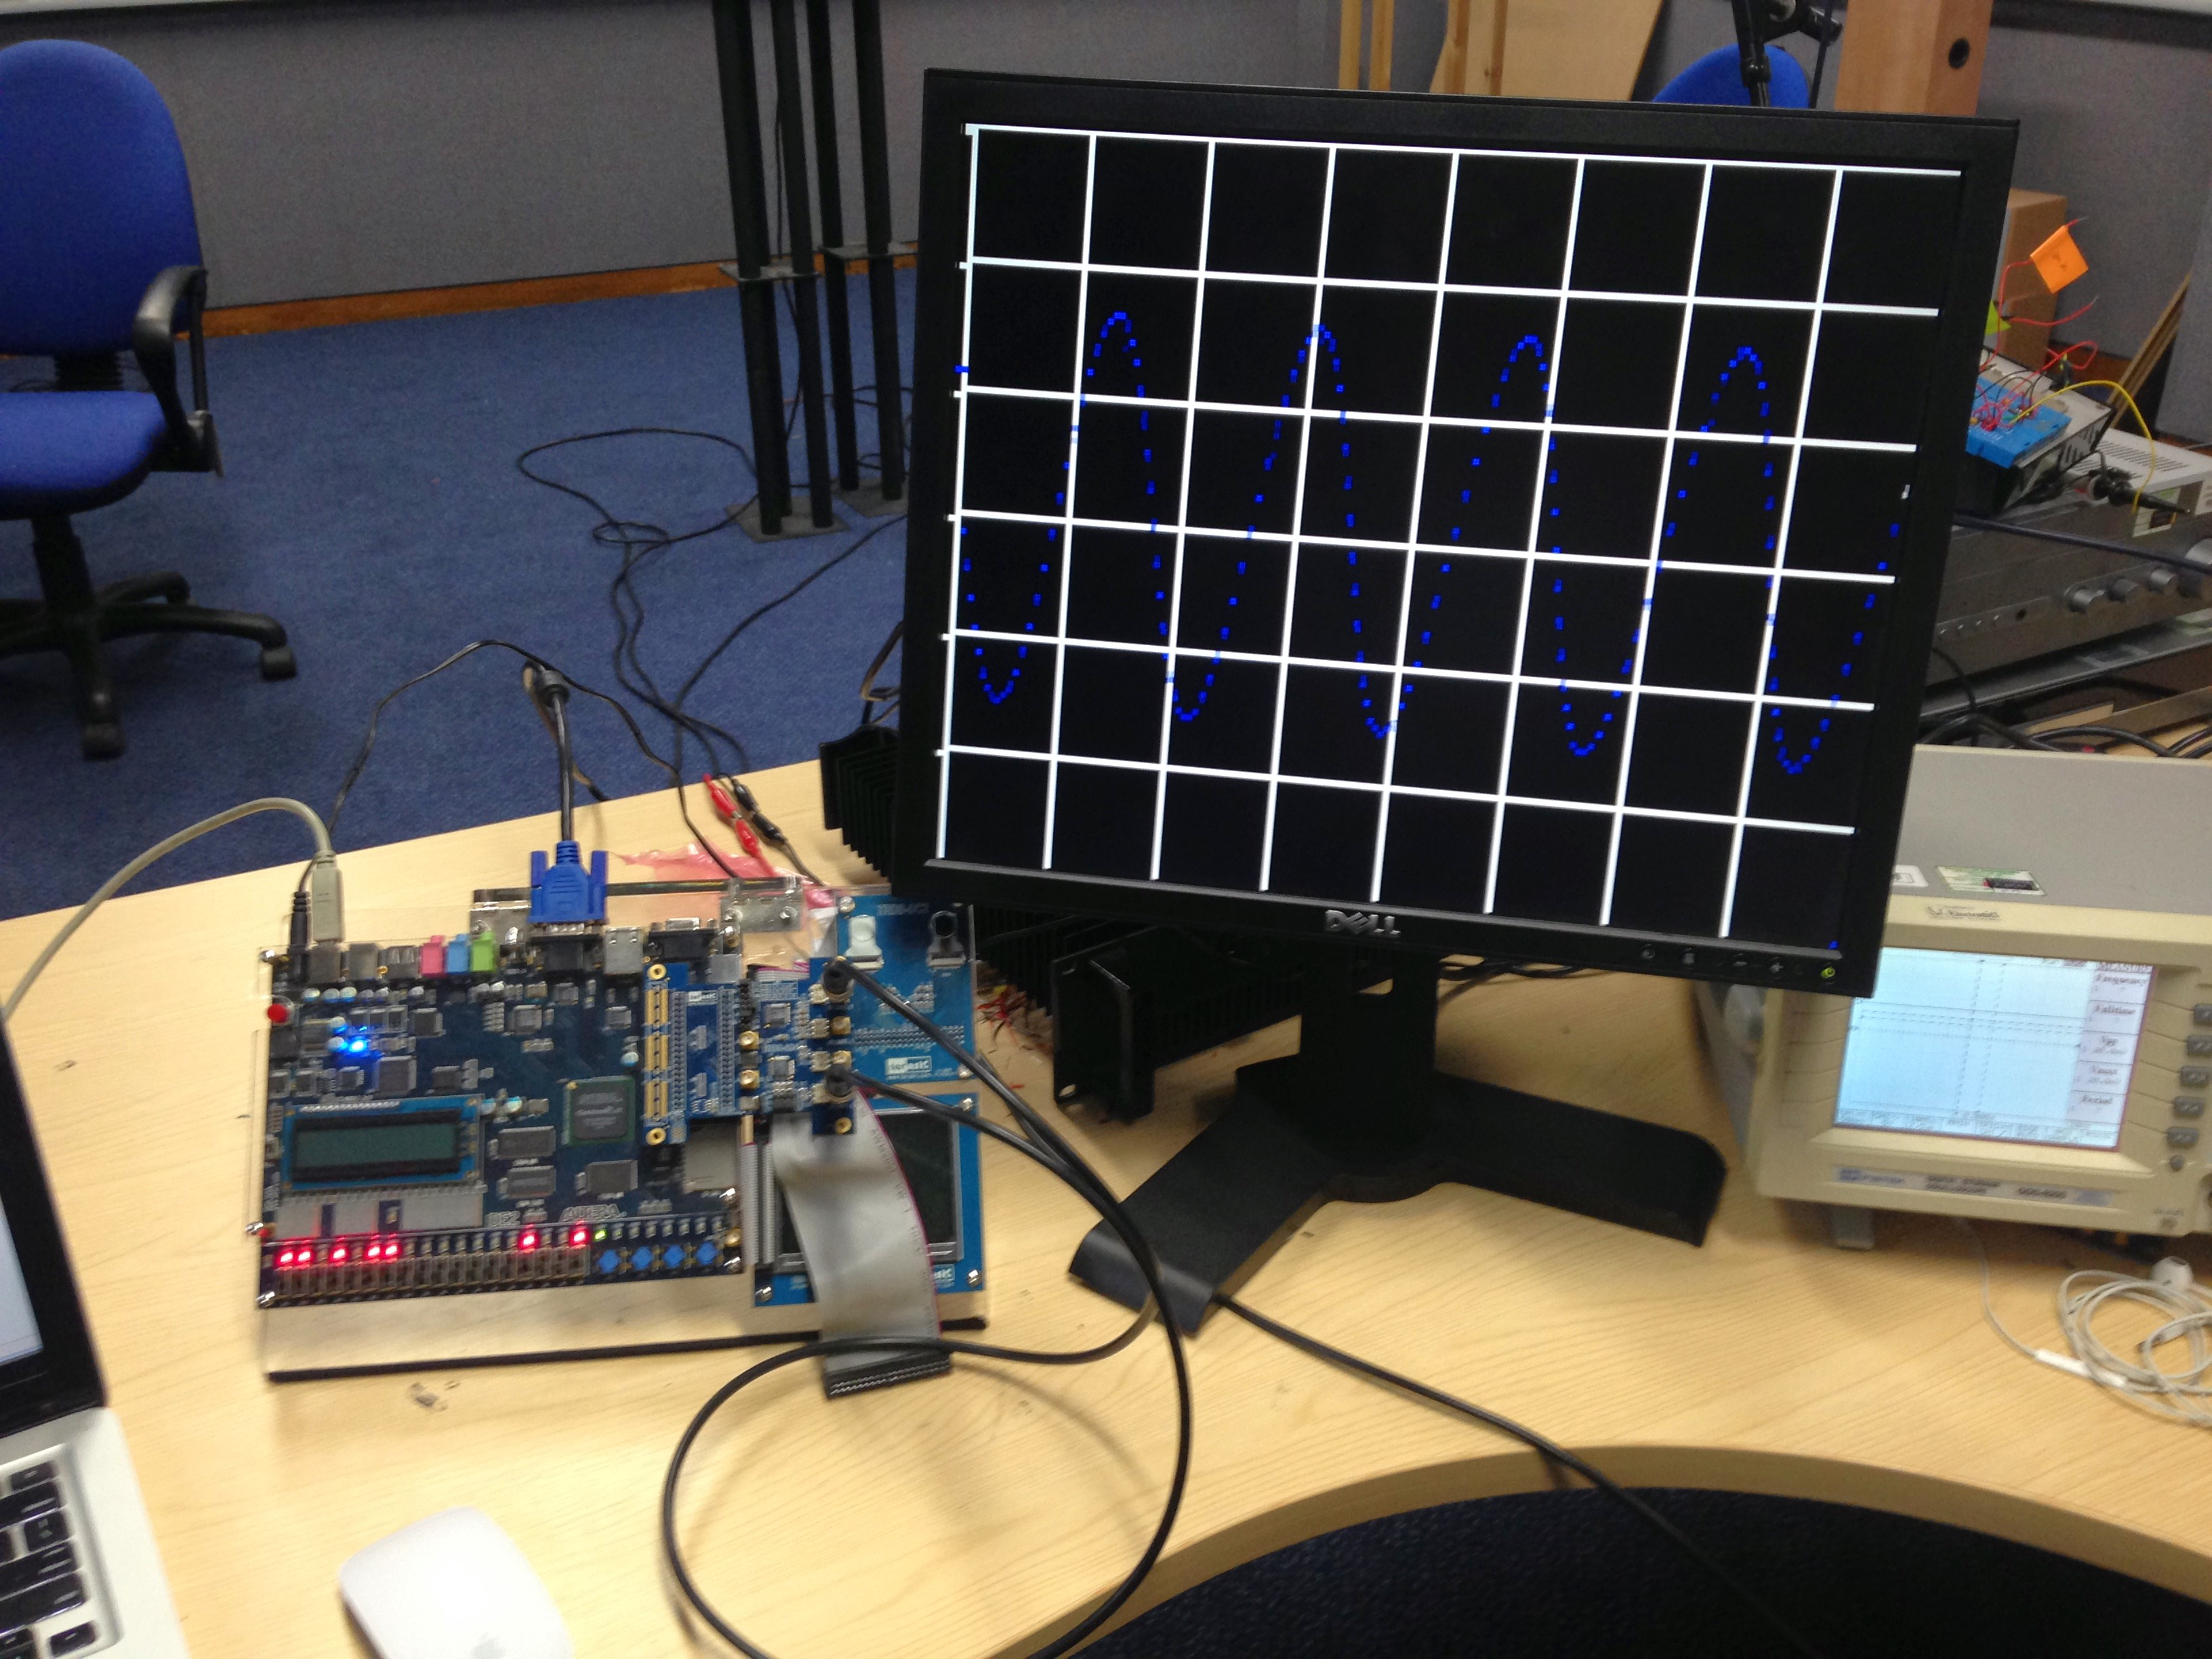
\includegraphics[scale = 0.15]{IMG_1388.JPG}
\captionof{figure}{This is the working result. The oscilloscope is reading the value from the generator}
}
\end{minipage}
\medskip
\end{center}


The board I was working on is called \textit{DE2-35}, which is an implementation of the Altera Cyclone\textregistered II FPGA chip 2C35 and the chip code is EP2C35F672C6. The board itself is designed for the purpose of evaluation and education and itself is built in with all sorts of basic components, \textit{i.e.} switches, push button, LCD screen, VGA modulator, GPIO pins etc. Beside from the FPGA board, I also used THDB\_ADA(ADA) daughter board for doing AD and DA conversion. Below is the specification of the chip and the AD-DA daughter board according to \cite{DE2UserManual} and \cite{addaman}.

\paragraph{The technical specification of the AD-DA daughter}

\begin{itemize}
    \item The AD channel is of 14-bit resolution and data rate up to 65 MSPS. Input volage range 2V p-p.
    \item The DA channel is of 14-bit resolution and data rate up to 125 MSPS. Output range 2V p-p.
\end{itemize}

\paragraph{The technical specification of the chip EP2C35F672C6 }
\begin{itemize}
    \item 33,216 LEs
    \item 105 M4K RAM blocks
    \item 483,840 total RAM bits
    \item 35 lembedded multipliers
    \item 4PLLs
    \item 475 user I/O pins
    \item FineLine BGA 672-pin package
\end{itemize}

For the software part of the project, a variety of software was used, I used \textit{quartus} for compiling the source code and downloading the program onto the board using JTAG. \textit{Git} for managing the development of the code. \textit{iverilog} for debugging. \textit{Matlab} for doing calculation and generating .mif file. \textit{verilog HDL} is the programming language.\\

The project itself is hosted at \textit{https://github.com/y1275963/vga\_basics}. With around 24 branches and 80 commits.\\


\section{Board Specification}
\subsection{Board Details}
For the board itself, I implemented a single route oscilloscope at the sampling frequency of 13.5Mhz or 27Mhz or 54Mhz and an arbitrary single route capable of generating wave at the base frequency of 97.66Khz and of the data point of 1024 points.%100
\subsection{The controlling method}

Below is the supported control method:

\begin{center}     
\begin{minipage}[t]{\linewidth}
%\label{fig:main}

{
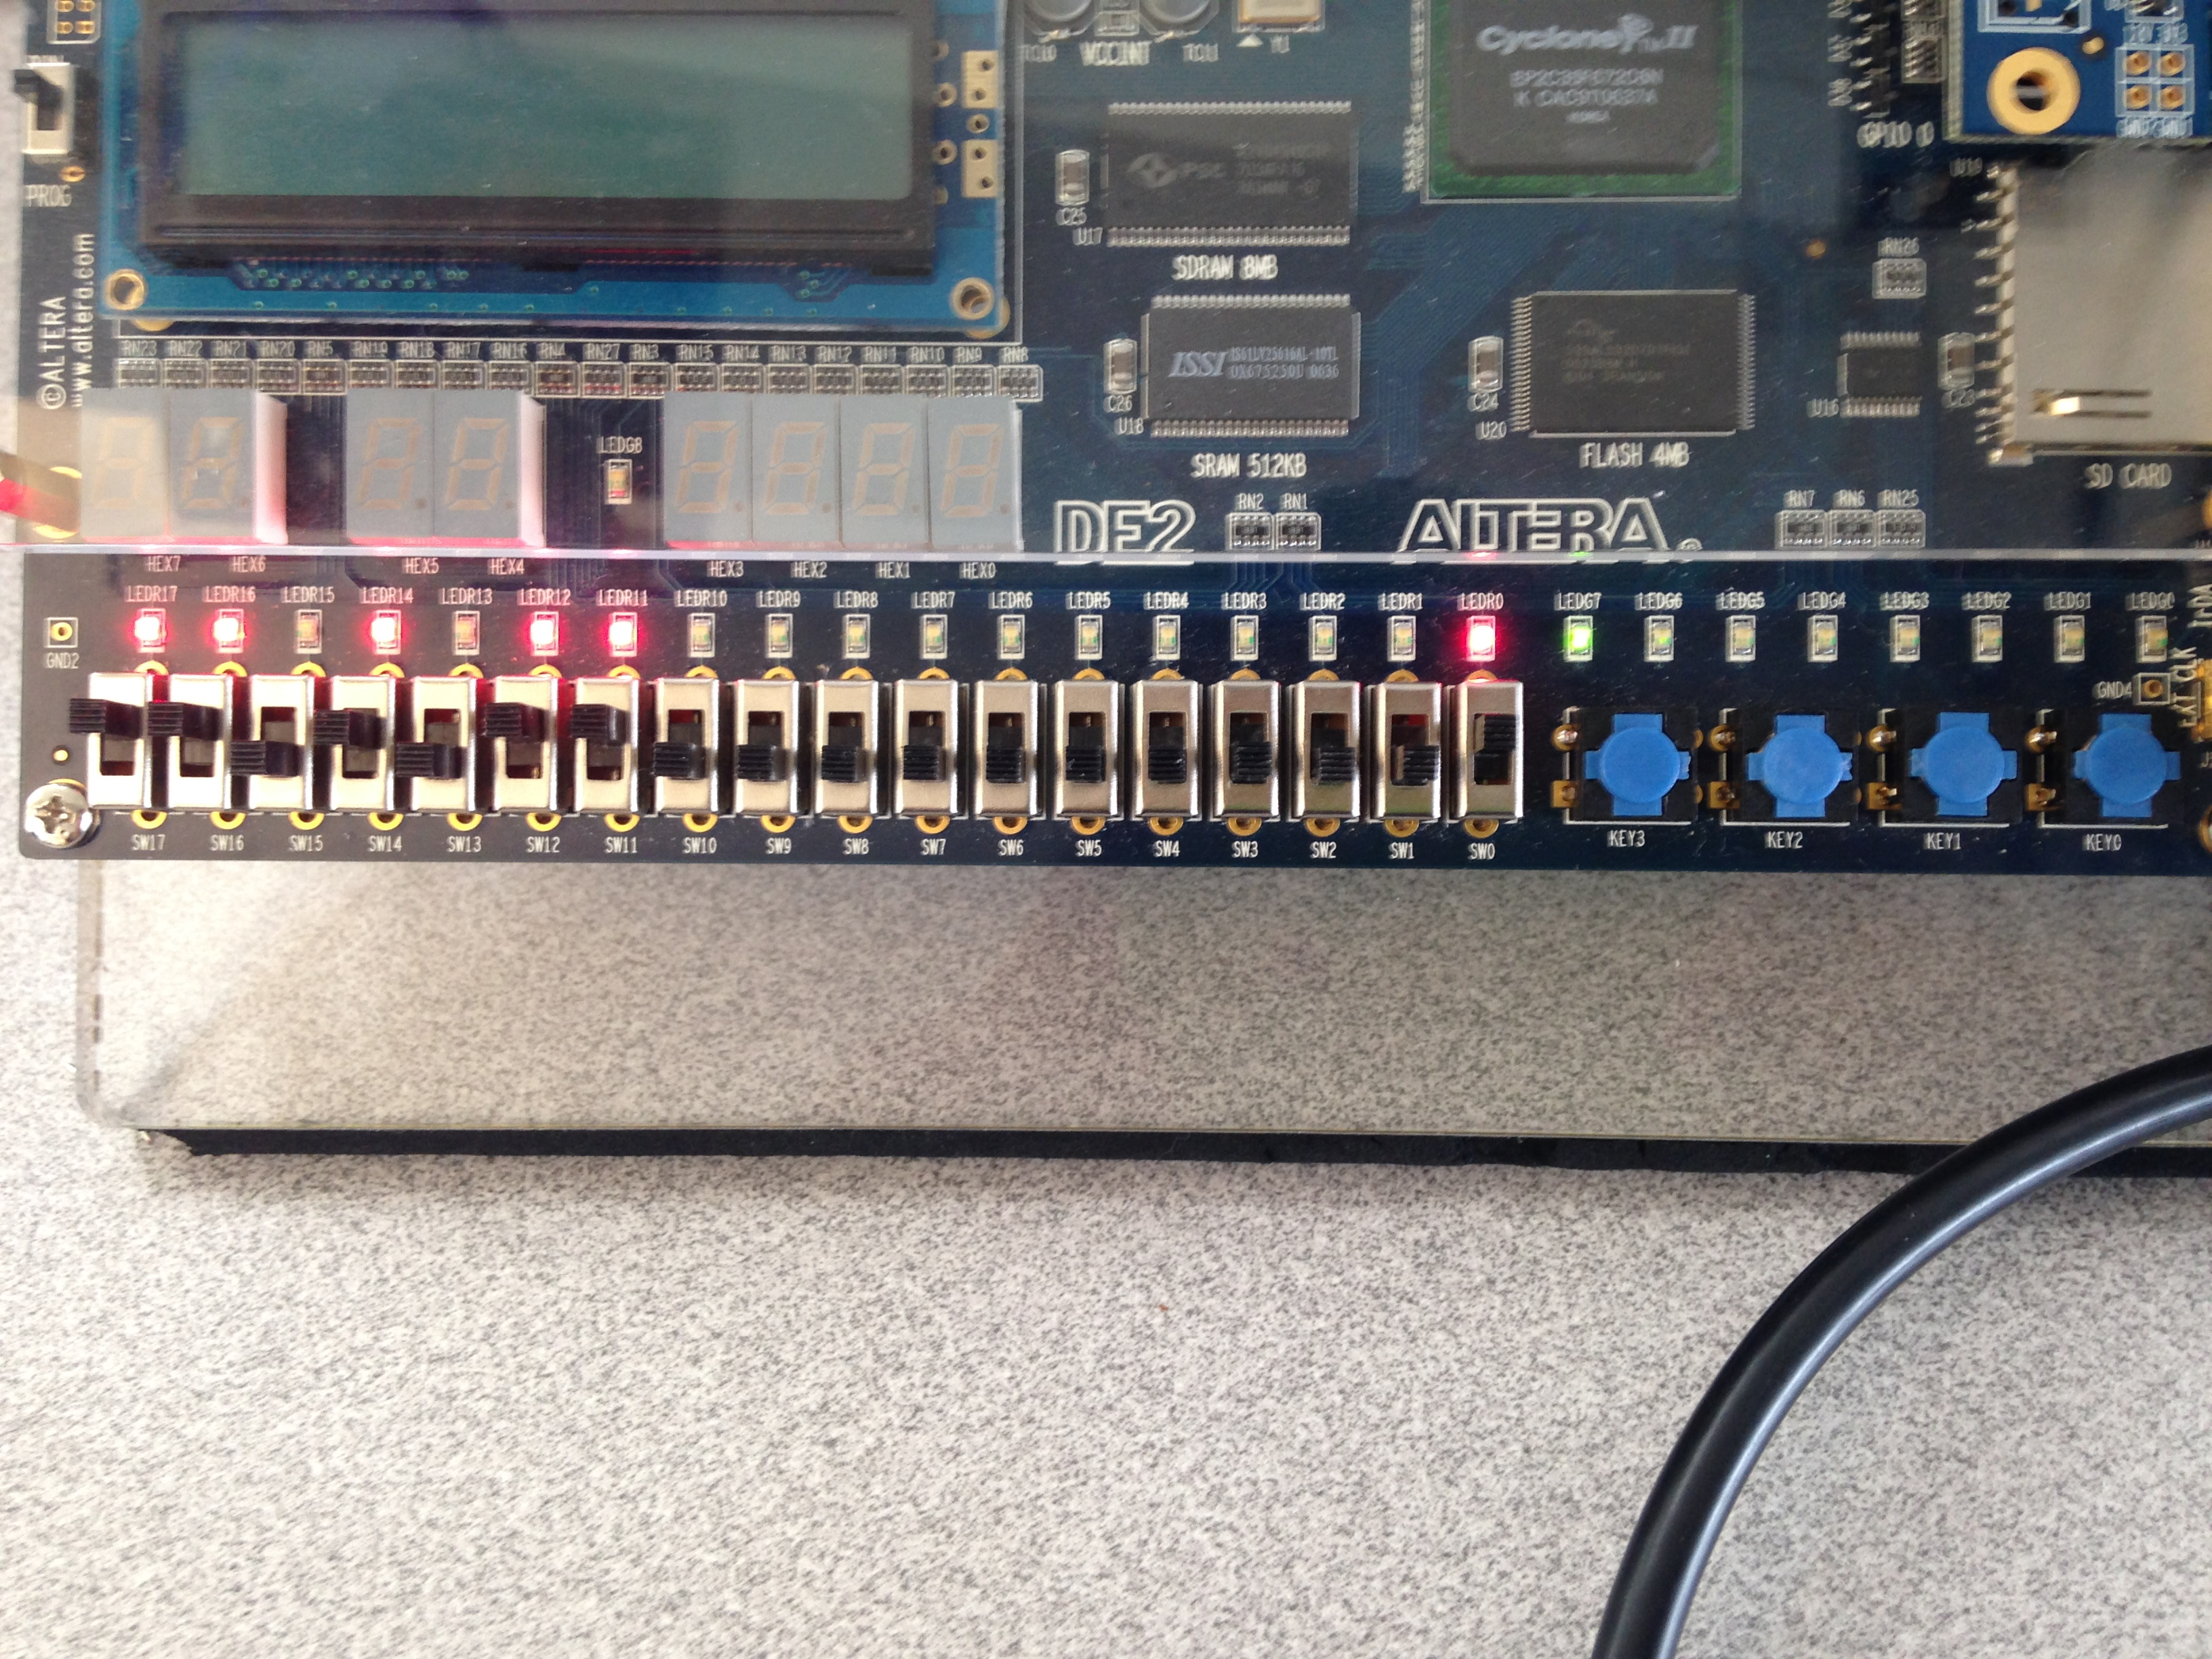
\includegraphics[scale = 0.08]{control.JPG}
\captionof{figure}{This is the overall view of the controlling method.}
}
\end{minipage}
\medskip
\end{center}

\begin{itemize}
    \item Switch 17:
    Switch for turning the monitor on and off.
    \item Switch 16:
    Switch for stoping refreshing the screen.
    \item Switch 15:
    Switch for letting the screen only show the background.
    \item Switch 13-14:
    Switches for changing time division by changing sampling frequency.
    
    Specifically:
    \begin{itemize}
        \item Switch 14 on, Switch 13 off:
        Sampling at 13.5Mhz.
        \item Switch 14 off, Switch 13 on:
        Sampling at 54Mhz.
        \item Switch 14 and 13 both on or off:
        Sampling at 27Mhz.        
    \end{itemize}
    \item Switch 11-12:
    Supporting for changing time division by changing sample rate.
    
    Specifically:
    \begin{itemize}
        \item Switch 12 and 11 both off:
        Sampling at normal speed.
        \item Switch 12 off and 11 on:
        Sampling at 1 time faster normal speed.
        \item Switch 12 on and 11 off:
        Sampling at 2 time faster normal speed.
        \item Switch 12 and 11 both on:
        Sampling at 3 time faster normal speed.
    \end{itemize}
    \item Switch 8-10:
    Supporting for shift the wave up.
    
    When switch is both off, no shift is made. And by turning it on or off, we can achieve shifting by 1,2,3,4,5,6,7 pixel above the central line.
    \item Switch 5-7:
    Supporting for shift the wave down.
    
    When switch is both off, no shift is made. And by turning it on or off, we can achieve shifting by 1,2,3,4,5,6,7 pixel below the central line.
    \item Switch 1-4:
    Supporting for changing the amplitude of the wave.
    
    The changing factor is done by a factor of 2. And switch 4-3 allowing for scale up, switch 2-1 allowing for scale down.
%    Specifically:
%    \begin{itemize}
%        \item Switch 4 and 3 both off:
%        Normal Amplitude.
%        \item Switch 4 off and 3 on:
%        Half of the original amplitude.
%        \item Switch 4 on and 3 off:
%        A quarter of the original amplitude.
%        \item Switch 4 and 3 both on:
%        $\frac{1}{8}$ of the original amplitude.
%    \end{itemize}
    
    \item Switch 0:
    Supporting for turning the function generator on and off.
    
    \item Push button 0:
    Supporting for changing the signal generator generated wave. The design itself allowing the program to record 4 sets of arbitrary waves before compiling the program. (Matlab program \ref{sec:correct} is provided for generating such wave) 
\end{itemize}

\subsection{The measuring method}
Below is the supported measuring method to get the data from the board.
\begin{itemize}
    \item The VGA monitor
    
    The monitor is the main source of information. We can use it to see the shape of the wave. Beside from this, because the regular grid is implemented as the background, measurement is made possible. Two measurement tables \ref{sec:fre} \ref{sec:amp} are provided for measuring the frequency and the amplitude of the wave. 
    \item The state machine debugger
    \begin{center}     
\begin{minipage}[t]{\linewidth}
%\label{fig:main}

{
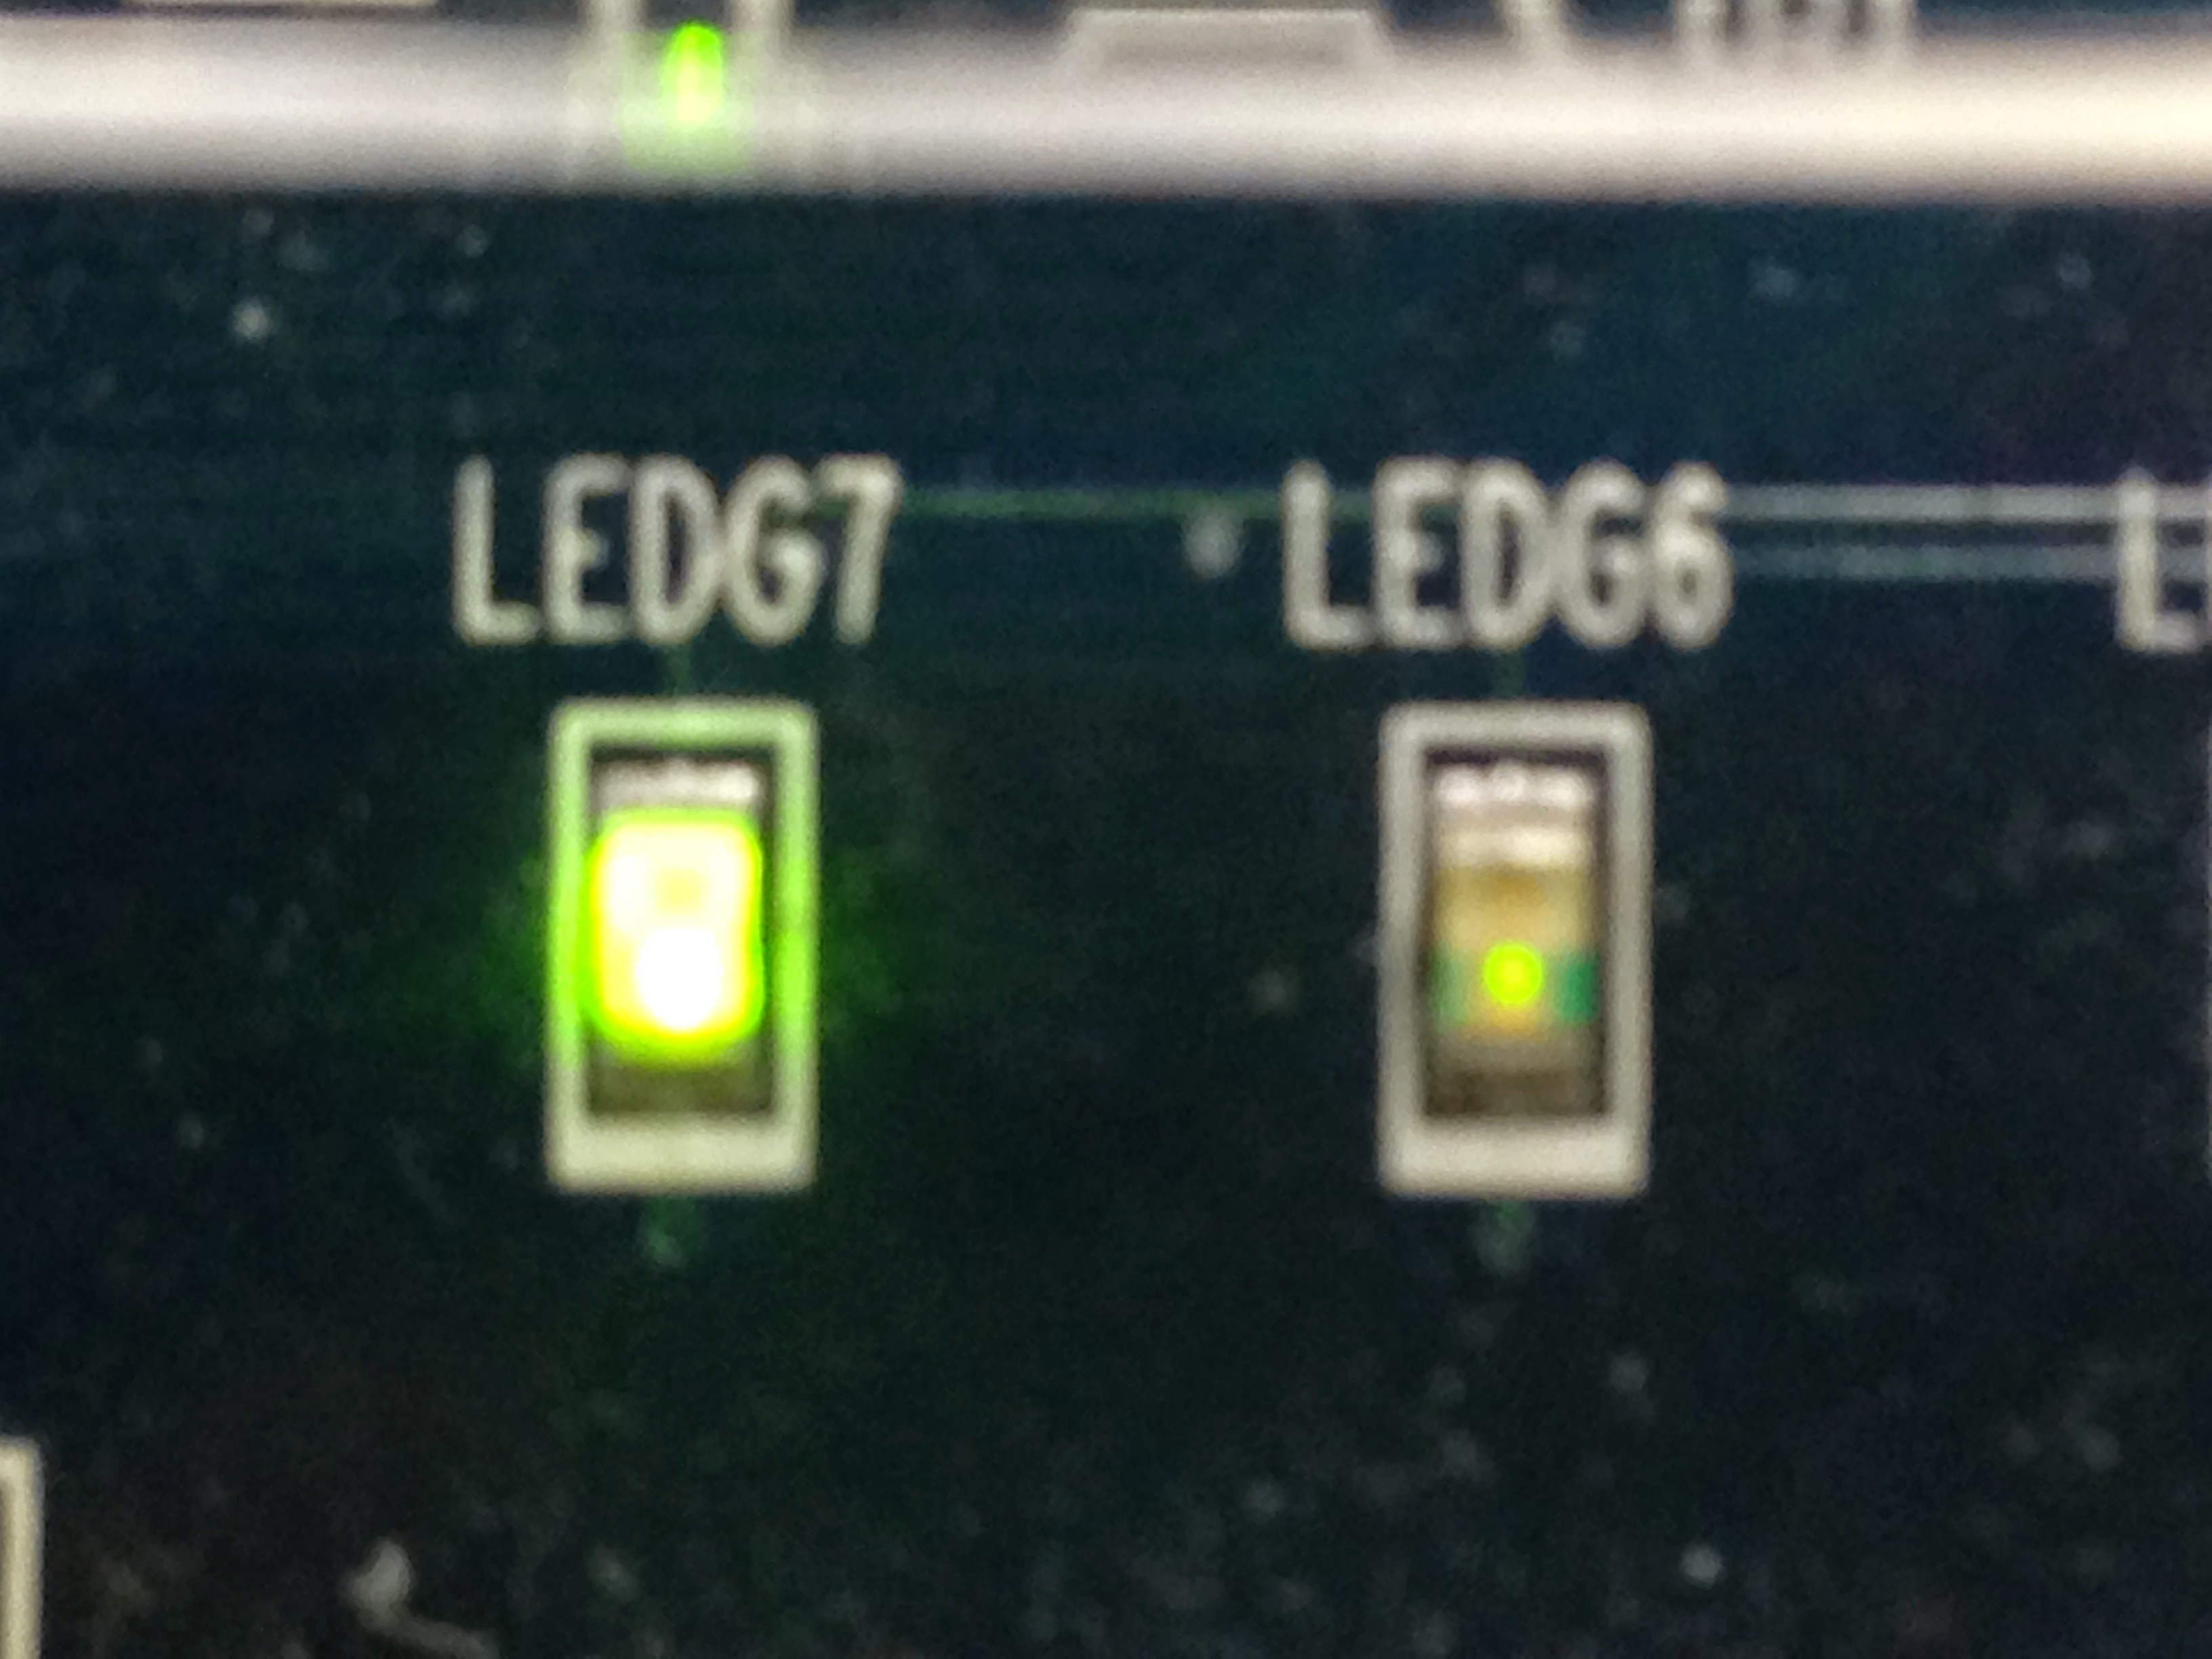
\includegraphics[scale = 0.05]{IMG_1386.JPG}
\captionof{figure}{This is the state indicator.}
}
\end{minipage}
\medskip
\end{center}

     LED Green 7 and 6 are implemented for indicating state machine's current state.( Image blow)

    
    Below is the meaning of the light:
    \begin{itemize}
        \item LED 7 is on, 6 is on, state 11:
         Meaning that the system is sampling.
         \item LDE 7 is on, 6 is off, state 10:
         Meaning that the system is delayed, to moderate the refresh rate down to around 50hz.
         \item LED 7 is off, 6 is on, state 01:
         Meaning that the system is drawing the wave from the RAM according to the sampled signal.
         \item LED 7 is off, 6 is off, state 00:
         Meaning that the system is clean the screen by redrawing a regular grid background.
         
    \end{itemize}  
      In reality, as we can see from the image above, because the system is the state of delay for most of its functioning time, we can see LED 7 is always on, and LED 6 is glimmering. Which means the system spent most of its time in delaying(state 10).
      \item Switch indicator
      
      The switch indicator is used to indicator which switch is on or off, as we can see from the image below:
      
    \begin{center}     
\begin{minipage}[t]{\linewidth}
%\label{fig:main}

{
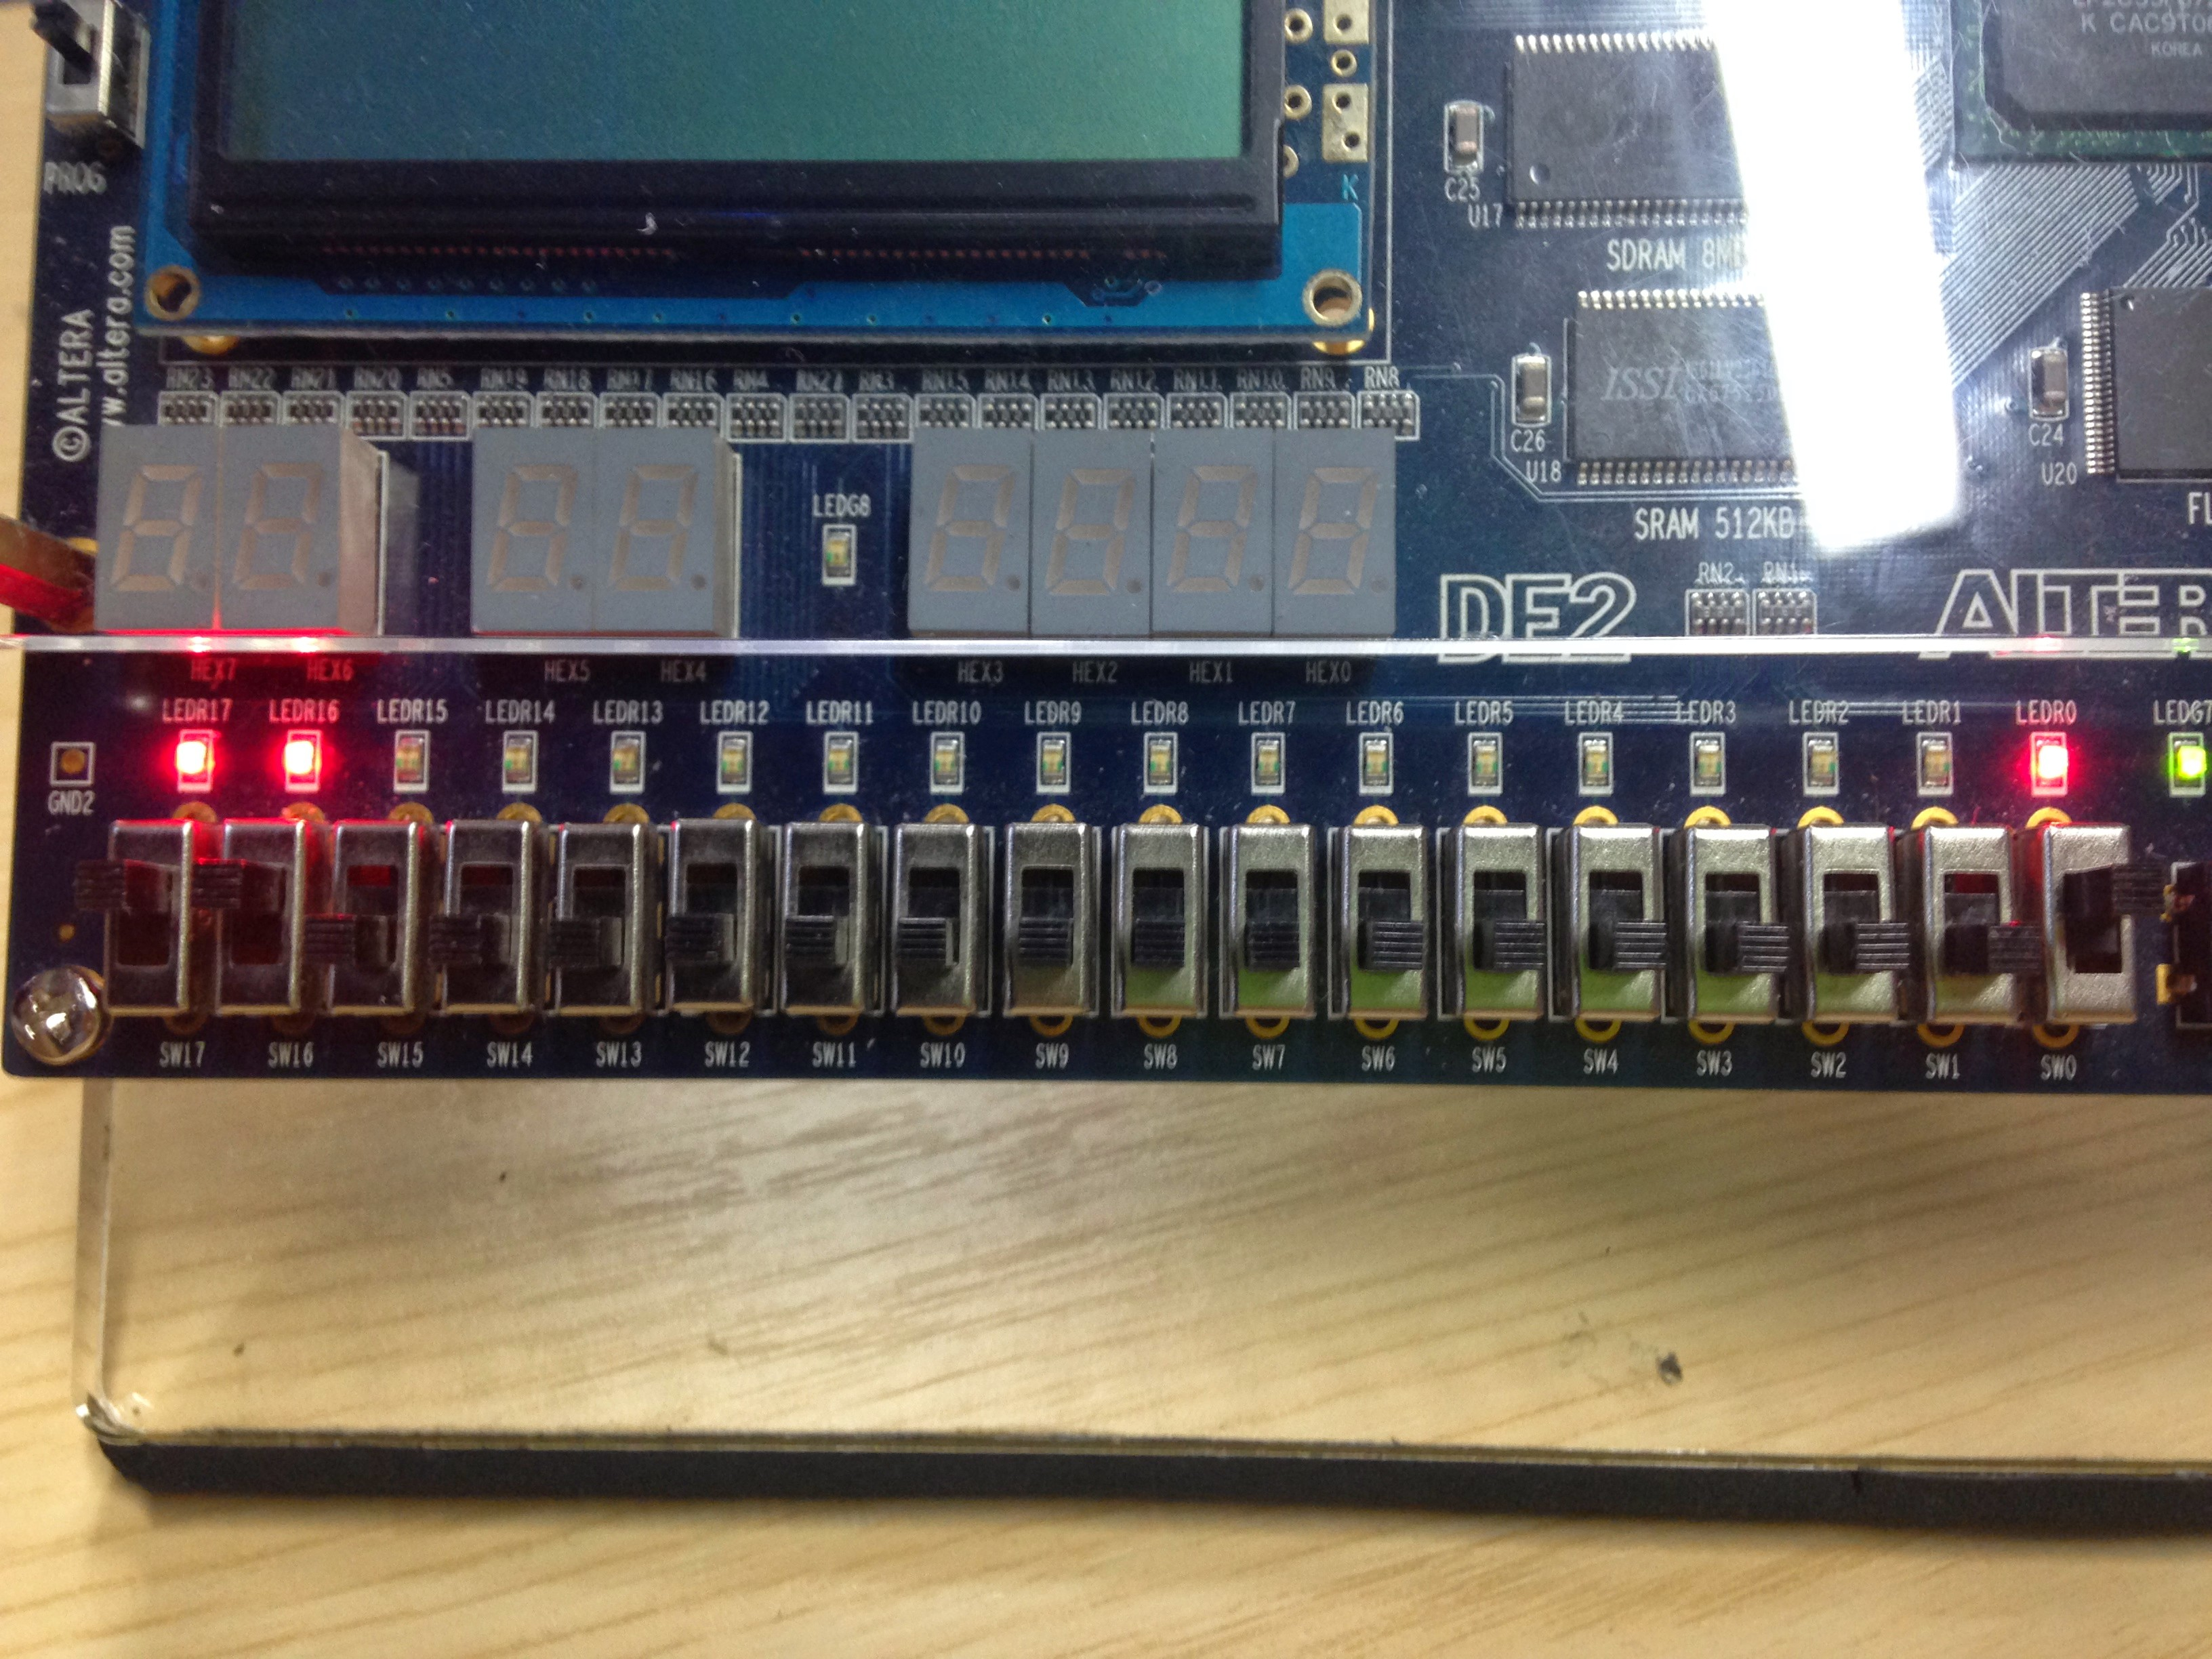
\includegraphics[scale = 0.1]{IMG_1387.JPG}
\captionof{figure}{This is switch indicator.}
}
\end{minipage}
\medskip
\end{center}
  
    
      
\end{itemize}

\subsection{The workflow}

This is the overall schematic chart:
\begin{center}
\begin{minipage}[t]{\linewidth}
%\label{fig:main}

{
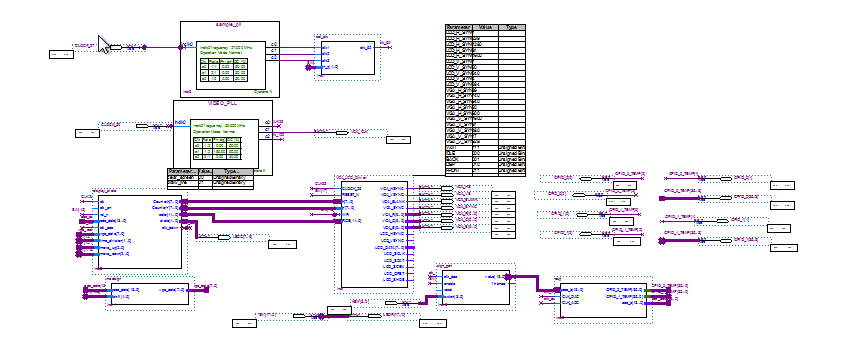
\includegraphics[scale = 0.5]{schematic.png}
\captionof{figure}{This is the workflow of the oscilloscope.}
}
\end{minipage}
\medskip
\end{center}

The board will execute two jobs simultaneously, below is the flowchart of the Oscilloscope:

\begin{center}
\begin{minipage}[t]{\linewidth}
%\label{fig:main}

{
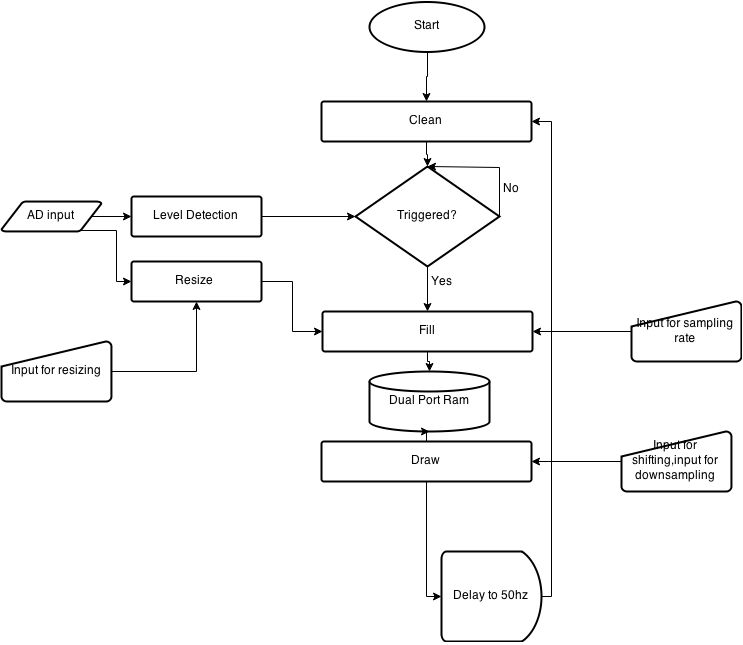
\includegraphics[scale = 0.5]{adchar.png}
\captionof{figure}{This is the workflow of the oscilloscope.}
}
\end{minipage}
\medskip
\end{center}
Below is the flowchart of the arbitrary function generator:
\begin{center}
\begin{minipage}[t]{\linewidth}
%\label{fig:main}

{
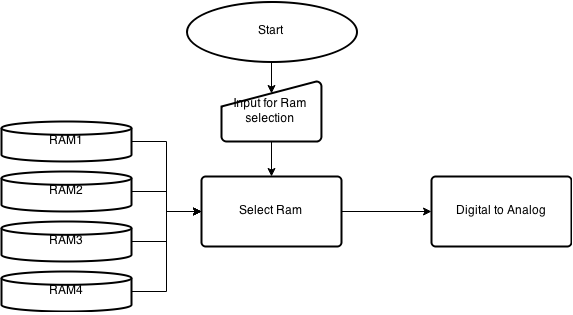
\includegraphics[scale = 0.6]{dachart.png}
\captionof{figure}{This is workflow of the function generator.}
}
\end{minipage}
\medskip
\end{center}


\section{Implementation Details}
\subsection{The Counter}
The counter is the building block of the entire project and it is used throughout the entire project. Below is the detailed list of the application of the counters:
\begin{itemize}
    \item In drawing process:
     Counters are used to provide VGA the pixel coordinates.
     \item In delay process:
     Counter is used to crate a delay to lower down the refresh rate.
     \item In sampling process and AD process:
    Counter is used to provide the RAM with memory index. A counter in sampling process also support downsampling the RAM.
\end{itemize}

To connect counters with state machine, all the counters are implemented with 2 input signals and 1 output signal:
\begin{itemize}
    \item enable: To start the counter
    \item reset: To reset the counter
    \item finished: indicate if the counter has finished one round or not.
\end{itemize}
\subsubsection{The basic Counter}
\label{sec:bascount}
All the counters are built on top the basic structure from the one blow:

\begin{lstlisting}[language=Verilog]
input clk;
input enable,reset;

output finished;
output reg [7:0] CounterX;
wire CounterXmaxed = (CounterX==8'd159); 
assign finished = (CounterXmaxed==1);

always @(posedge clk)
begin
	if(reset == 1)
		CounterX <= 0;
	else
	begin
	if(CounterXmaxed)
	  	CounterX <= 0;
	else if(enable == 1)
	  	CounterX <= CounterX + 1;
	 end
end
\end{lstlisting}

By setting the value of the maximum value of the counter, we can manage to let the counter counts from 0 to its max value according to the clock. And the finished signal is emitted right at the moment the counter reach its maximum value.

\subsubsection{Jumping Counter}
\label{sec:jumcount}

The downsampling is implemented by downsampling the output of the RAM instead of downsampling the output from the AD converter.

To support the downsampling, we simply change the increment factor of the counter and hence we change the RAM address we are going to access, below is an example of the jumping counter:
 
\begin{lstlisting}[language=Verilog]
input [1:0] time_division;
wire [2:0] read_time_division = time_division + 1; // to avoid 0, start from 1

output reg [7:0] read_CounterX;

wire read_CounterX_Maxed = (read_CounterX >= 8'd1023);

always @(posedge clk)
begin
	if(reset == 1)
		read_CounterX <= 0;
	else
	begin
	if(read_CounterX_Maxed)
	  	read_CounterX <= 0;
	else if(enable == 1)
	  	read_CounterX <= read_CounterX + read_time_division + 1;
	 end
end
\end{lstlisting}
\subsubsection{Counter on top of the Counter}
\label{sec:coucount}

To support providing $(x,y)$ coordinators for the VGA module while cleaning the whole screen, a Y counter is built on top of a X counter, blow is the example:
\begin{lstlisting}[language=Verilog]

input clk;
input reset,enable;

output reg [7:0] CounterX,CounterY;
output finished;

wire [14:0] address;

wire CounterXmaxed = (CounterX==8'd159); // 159
wire CounterYmaxed = (CounterY==8'd119); // 119
assign finished = ((CounterXmaxed == 1) && (CounterYmaxed == 1));

assign address = CounterX + CounterY * 160;

always @(posedge clk)
begin
	if(reset == 1)
		CounterX <= 0;
	else
	begin
	if(CounterXmaxed)
	  CounterX <= 0;
	else if(enable == 1)
	  CounterX <= CounterX + 1;
	end
end

always @ (posedge clk)
begin
	if(reset == 1)
		CounterY <= 0;
	else
	begin
		if(CounterXmaxed == 1)
\end{lstlisting}
\subsubsection{iverilog output for testing}
Because we need a reliable counter to make sure it goes exactly as we wish, \textit{iverilog} is used for testing, below is its output:

This is snapshot of the testing from the basic counter:
\begin{verbatim}
ticket:23370    ,enable:1       ,reset:0        ,x:155  ,finished :0
ticket:23380    ,enable:1       ,reset:0        ,x:156  ,finished :0
ticket:23390    ,enable:1       ,reset:0        ,x:157  ,finished :0
ticket:23400    ,enable:1       ,reset:0        ,x:158  ,finished :0
ticket:23410    ,enable:1       ,reset:0        ,x:159  ,finished :1
ticket:23420    ,enable:1       ,reset:0        ,x:  0  ,finished :0
\end{verbatim}
Below is the snapshot of the testing from the jumping counter:
\begin{verbatim}
ticket:23950    ,enable:1       ,reset:0        ,x:147  ,finished :0
ticket:23960    ,enable:1       ,reset:0        ,x:150  ,finished :0
ticket:23970    ,enable:1       ,reset:0        ,x:153  ,finished :0
ticket:23980    ,enable:1       ,reset:0        ,x:156  ,finished :0
ticket:23990    ,enable:1       ,reset:0        ,x:159  ,finished :1
ticket:24000    ,enable:1       ,reset:0        ,x:  0  ,finished :0
ticket:24010    ,enable:1       ,reset:0        ,x:  3  ,finished :0
ticket:24020    ,enable:1       ,reset:0        ,x:  6  ,finished :0
\end{verbatim}


Below is the snapshot of the testing from the xy counter:
\begin{verbatim}
ticket:575970   ,enable:1       ,reset:0        ,x:155  ,y:119  ,finished :0
ticket:575980   ,enable:1       ,reset:0        ,x:156  ,y:119  ,finished :0
ticket:575990   ,enable:1       ,reset:0        ,x:157  ,y:119  ,finished :0
ticket:576000   ,enable:1       ,reset:0        ,x:158  ,y:119  ,finished :0
ticket:576010   ,enable:1       ,reset:0        ,x:159  ,y:119  ,finished :1
ticket:576020   ,enable:1       ,reset:0        ,x:  0  ,y:  0  ,finished :0
ticket:576030   ,enable:1       ,reset:0        ,x:  1  ,y:  0  ,finished :0
ticket:576040   ,enable:1       ,reset:0        ,x:  2  ,y:  0  ,finished :0
ticket:576050   ,enable:1       ,reset:0        ,x:  3  ,y:  0  ,finished :0
\end{verbatim}

Below is the example of the test bench:
\begin{lstlisting}[language=Verilog]
module ramfill_tb;

// module ramfill(clk_adc,enable,reset,finfished,adc_data,vga_data,CounterX);
reg clk;
wire [7:0] CounterX;
reg enable,reset;
wire finished;

vga_sin u0(
	.clk(clk), 
	.reset	(reset),
	.enable (enable),
	.finished (finished), 
	.CounterX	(CounterX));

always  
   #5 clk = ~clk; 
    
initial begin
	reset = 0;
	enable = 0;
	clk = 1;

	#10 reset = 1;//after 10 tickets
	#10 reset = 0;//then after 10 tickets,reset is set 1 after reset == 1 is kept for 10 tickets
	#10 enable = 1;
	#20000 reset = 1;//try again
	#200 reset = 0;
	#2000 enable = 1;
	#2000 enable = 0;
	#200 reset = 0;
	#25 $finish; 
end


initial  begin
    $monitor("ticket:%g\t,enable:%b\t,reset:%b\t,x:%d\t,finished :%b",$time,enable,reset,CounterX,finished); 
end 

endmodule
\end{lstlisting}

\subsection{The RAM}
It would be good if we can write some test bench with RAM, but because it is a Mega function and I cannot find a way to compile it.


The RAM is used throughout the project as well, below is a list of its usage:
\begin{itemize}
    \item In clean process: A RAM is used to provide the grid image which is going to be drawn.
    \item In sampling process: A RAM is used to store the sampling information
    \item In drawing process: The same RAM is used to retrieve stored sampled data.
    \item In DA process: 4 RAMs are used to store the pro recored wave information. 
    \end{itemize}
\subsubsection{One Port reading only RAM}
\label{sec:siram}
This is the basic usage of the RAM, and the purpose of this is simply to get the initialing memory information from the RAM, below is an example:
\begin{lstlisting}[language=Verilog]
wire rambuffer;
ram_background ram_entity(
 	.address(address),
 	.clock(clk),
 	.wren(1'b0),
 	.q(rambuffer));
endmodule
\end{lstlisting}
The \textit{address} nets are defined by other counters.

\subsubsection{Dual Port RAM}
\label{sec:duram}
That is hardest part of the entire project, and the natural way of doing so is by using a FIFO mega function \cite{fifo}. But because \textit{quartus} only provide fixed length FIFO and due to various other reasons, I cannot figure out a right way of stopping the FIFO from overflow, an image is provided to demonstrate the problem:


\begin{minipage}[t]{\linewidth}
%\label{fig:main}

{
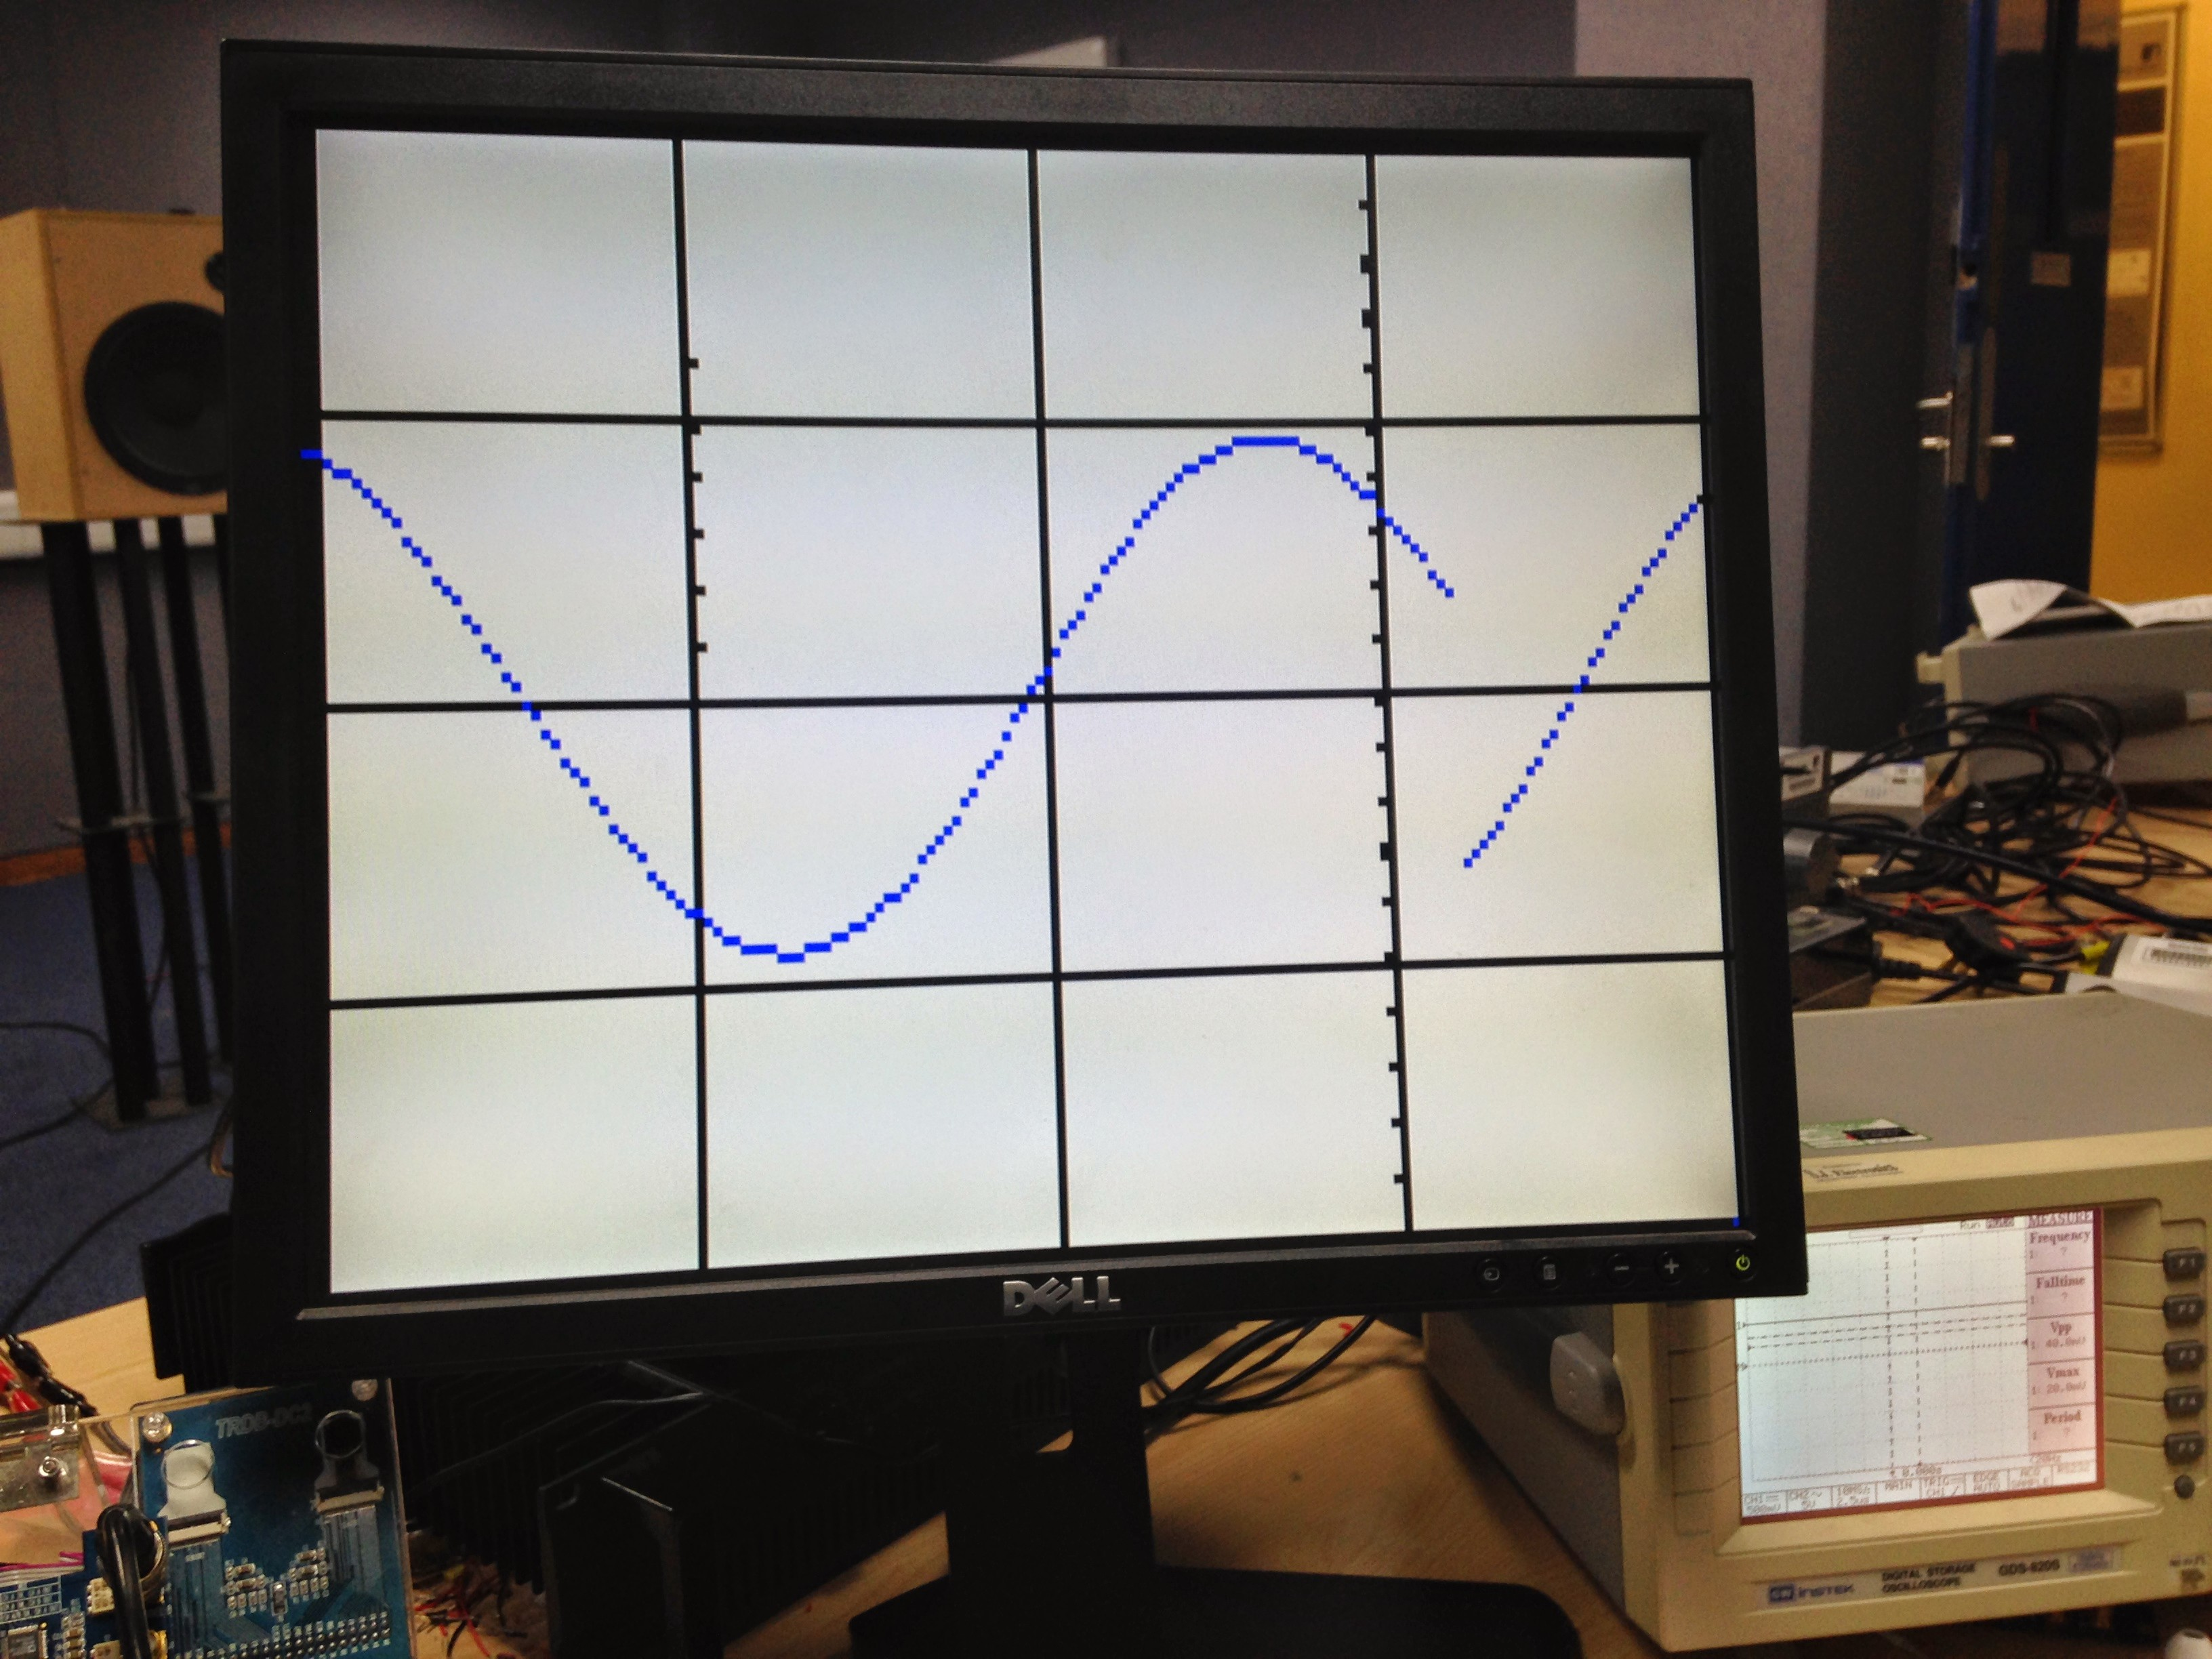
\includegraphics[scale = 0.1]{IMG_1389.JPG}
\captionof{figure}{There is a periodic unsolvable overflow problem at each image when using FIFO.}
}
\end{minipage}
\medskip

And a dual port asynchronous memory is a core component of the entire design, it is used to link the AD sampled data to the image on the screen. Its difficulties are listed as follows:
\begin{itemize}
    \item It must support one reading port and one writing port running at different speed.
    \item It is written at writing speed, but at the reading cycle the finishing of the writing must be able to be detected. And the clock shift is unknown. 
    \item There is a trigging mechanism in between, so the port is not being written periodically.
\end{itemize}

And the solution is the example below:
\begin{lstlisting}[language=Verilog]
// sync clocks
reg prolong_finished = 0;
always @(posedge w_finished) // flip flop
begin
	prolong_finished = prolong_finished + 1;
end

reg previous_signal;
reg r_finished;
always @(posedge clk) 
begin
	previous_signal <= prolong_finished; 
	r_finished <= previous_signal ^ prolong_finished;
	// or with its previous value.
end
\end{lstlisting}

The writing finished signal will change the state of a flip-flop register, and the reading clock will be constantly detecting the level of the register and when  it detects the difference it will output a reading finished signal.

By doing so, I successfully made the writing finished clock readable from the reading cycle. Therefor, the state machine will be able to detect if the sampling is finished at a different clock.\\


Below is a simulation result:

\begin{minipage}[t]{\linewidth}
%\label{fig:main}

{
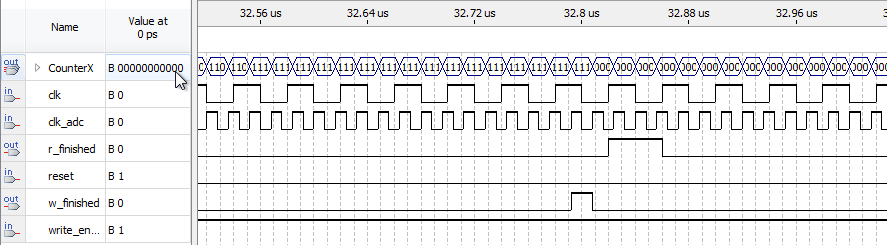
\includegraphics[scale = 0.5]{dualram.png}
\captionof{figure}{This is simulation of the synchronization of the finished clock.}
}
\end{minipage}
\medskip

\subsection{The State Machine}
\label{sec:state}
The state machine runs at the pixel refresh rate, which is 25Mhz, and it is the main block of the whole project. \\


The implementation of state machine goes as the following, Once a state is finished a new state will be defined. And the state machine changes its state accordingly. 

For all the states, it always goes from enabling its module and reseting all the others modules by using \textit{enable}, \textit{reset} and \textit{finished}. \\


It is separated in 4 stages:
\begin{itemize}
    \item clean:
    Call the clean module to clean the screen, and it goes to \textit{fill} module when it is finished.
    \item fill:
    Call the Sampling module to write memory to the RAM, and it goes to \textit{draw} module when it is finished. Notice that the state machine detects the state of the filling module at 25Mhz but the filling module itself runs at sampling frequency.
    \item draw:
    Call the drawing module to draw the memory according to the RAM, and it goes to \textit{delay} module when it is finished.
    \item delay:
    Call the delay module to delay the whole process, and it goes to \textit{clean} module when it is finished.
\end{itemize}




Below is the snapshot code of the state machine:
\begin{lstlisting}[language=Verilog]

always @ (posedge clk)
begin
	if(rst_n == 1)
		state <= clear_screen;
	else
		state <= next_state;
end

always @ * // combinational circuit
	case(state)
		clear_screen:
		begin
			enable_clear = 1;
			reset_clear = 0;

			enable_sin = 0;
			reset_sin = 1;

			enable_delay = 0;
			reset_delay = 1;

			enable_fill = 0;
			reset_fill = 1;

			CounterX = CounterX_clear;
			CounterY = CounterY_clear;
			color = color_clear;
			if(finished_clear == 0)
				next_state = clear_screen;
			else
				next_state = fill;
		end
		fill:
		begin
			enable_fill = 1;
			reset_fill = 0;		

			enable_clear = 0;
			reset_clear = 1;

			enable_sin = 0;
			reset_sin = 1;

			enable_delay = 0;
			reset_delay = 1;

			CounterX = 8'bzzzz_zzz;
			CounterY = 8'bzzzz_zzz;
			color = 12'bzzz_zzz_zzz_zzz;

			if(finished_fill == 0)
				next_state = fill;
			else
				next_state = draw_line;			

		end
		draw_line:
		begin
			enable_sin = 1;
			reset_sin = 0;

			enable_delay = 0;
			reset_delay = 1;

			enable_clear = 0;
			reset_clear = 1;

			enable_fill = 0;
			reset_fill = 1;			

			CounterX = CounterX_sin;
			CounterY = ram_output + move_down - move_up;
			color = color_sin;
			if(finished_sin == 0)
				next_state = draw_line;
			else
				next_state = do_nothing;
		end
		do_nothing:
		begin
			enable_delay = 1;
			reset_delay = 0;

			enable_clear = 0;
			reset_clear = 1;

			enable_sin = 0;
			reset_sin = 1;

			enable_fill = 0;
			reset_fill = 1;			

			CounterX = 8'bzzzz_zzz;
			CounterY = 8'bzzzz_zzz;
			color = 12'bzzz_zzz_zzz_zzz;
			if(finished_delay == 0)
				next_state = do_nothing;
			else	
				next_state = clear_screen;
		end 
	endcase
\end{lstlisting}
 
\subsection{The Trigger}
\label{sec:trigger}
The trigger detects the input signal and emit an enabling signal to start the sampling, two mechanism is implemented and tested.


The first one is simply to use the most significant bit of the input signal:

\begin{lstlisting}[language=Verilog]
wire last_bit_data = adc_data[13];
reg previous_adc_data;
// wait until trigger happen
always @ (posedge clk_adc)
begin
	previous_adc_data <= last_bit_data;
	if(enable == 1)
	begin
		if((last_bit_data ^ previous_adc_data) == 1) // unchanged until enable returns to 0.
			write_enable <= 1;
	end
	else
		write_enable <= 0;
end
\end{lstlisting}

and according to \cite{trigger}, I implemented a different design:

\begin{lstlisting}[language=Verilog]

always @ (posedge clk_adc)
begin
	if(enable == 1)
	begin
		if(Trigger == 1) // unchanged until enable returns to 0.
			write_enable <= 1;
	end
	else
		write_enable <= 0;
end

reg Threshold1, Threshold2;
always @(posedge clk_adc) Threshold1 <= (adc_data>=14'b10_000_000_000_000);
always @(posedge clk_adc) Threshold2 <= Threshold1;

wire Trigger = Threshold1 & ~Threshold2;  // if positive edge, trigger! 
\end{lstlisting}

Both of the design work, but according to the performance, the last one works better than the former.\\

Clearly, we can pin out the \textit{trigger} signal and therefor enable the external trigger signal.
\subsection{PLL}

PLLs are used to change the clock,

The first one receive signal from 50Mhz and generate 3 signals. Two for VGA module, which are 25Mhz and 25Mhz with 180 degree shift. One for DA module which is 100Mhz.

\begin{minipage}[t]{\linewidth}
%\label{fig:main}

{
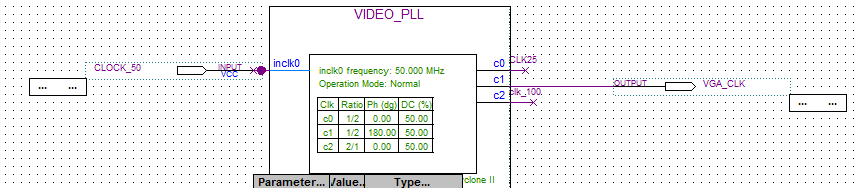
\includegraphics[scale = 0.5]{pll1.png}
\captionof{figure}{This is the first PLL.}
}
\end{minipage}
\medskip

The second one receive signal from 27Mhz and generate 3 signals, all of them are used for providing a adjustable sampling rate, which are 13.5Mhz, 27Mhz and 54Mhz. 

\begin{minipage}[t]{\linewidth}
%\label{fig:main}

{
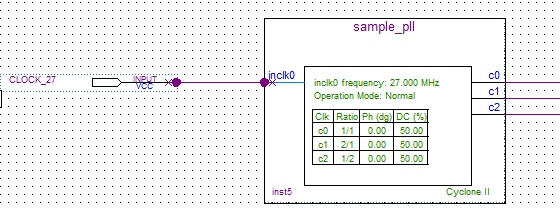
\includegraphics[scale = 0.5]{pll2.png}
\captionof{figure}{This is the second PLL.}
}
\end{minipage}
\medskip

\subsection{University Provided modules}
\subsubsection{The VGA Adaptor Module}
\label{sec:vga}
VGA module is used to connect the board with the monitor, below is the schematic snapshot:

\begin{minipage}[t]{\linewidth}
%\label{fig:main}

{
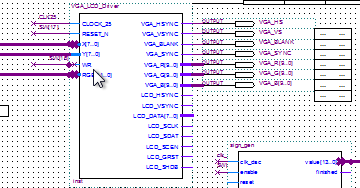
\includegraphics[scale = 1]{vga.png}
\captionof{figure}{This is the VGA Adaptor.}
}
\end{minipage}
\medskip

Although it is a different module, but I use it according to this table \cite{vgaadaptor}.

\subsubsection{The AD-DA Adaptor Module}
\label{sec:adda}
AD-DA adaptor module provide a interface for me to control the AD-DA converter. Below is the snapshot of its schematic design:

\begin{minipage}[t]{\linewidth}
%\label{fig:main}

{
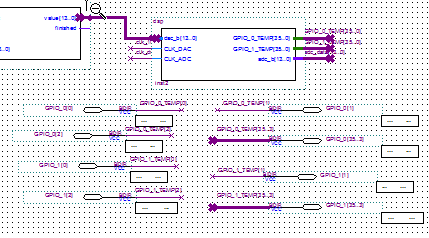
\includegraphics[scale = 1]{adda.png}
\captionof{figure}{This is the AD\-DA Adaptor.}
}
\end{minipage}
\medskip

\subsection{Matlab code}

Aside from the \textit{verilog HDL} code, there is roughly $1.5\%$ Matlab code.   
\subsubsection{Matlab code for RAM initialization file} 
\label{sec:correct}
Because RAM need to read its initialing file, two Matlab files are written, one is to generate the background and another one is to generate wave for DA converter.\\

The one below is for generating the background, it is able to convert an image into RAM initializing file:
\begin{lstlisting}[language=Matlab]
function imgscaled = miffilegen(infile, outfname, numrows, numcols)
%miffilegen('photo.jpg','test.mif',120,160) generate black and white image.

img = imread(infile);
bw = im2bw(img,0.5);

imgresized = imresize(bw, [numrows numcols]);

[rows, cols, ~] = size(imgresized);

imgscaled = imgresized;
imshow(imgscaled*16);

fid = fopen(outfname,'w');

fprintf(fid,'-- %3ux%3u 1bit image color values\n\n',rows,cols);
fprintf(fid,'WIDTH = 1;\n');
fprintf(fid,'DEPTH = %4u;\n\n',rows*cols);
fprintf(fid,'ADDRESS_RADIX = UNS;\n');
fprintf(fid,'DATA_RADIX = UNS;\n\n');
fprintf(fid,'CONTENT BEGIN\n');
imshow(imgscaled);
count = 0;
for r = 1:rows
    for c = 1:cols
%         red = uint16(imgscaled(r,c,1));
%         green = uint16(imgscaled(r,c,2));
%         blue = uint16(imgscaled(r,c,3));
%         color = red*(256) + green*16 + blue;
        fprintf(fid,'%4u : %4u;\n',count, imgscaled(r,c));
        count = count + 1;
    end
end
fprintf(fid,'END;');
fclose(fid);

return
\end{lstlisting}

The code is modified to be able to generate an image directly from Matlab's array for accuracy, and the standard background is a 160 * 120 image shown blow:
\begin{center}
\begin{minipage}[t]{\linewidth}
%\label{fig:main}

{
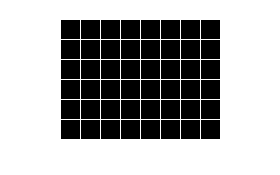
\includegraphics[scale = 1]{temp.png}
\captionof{figure}{This is the background image.}
}
\end{minipage}
\medskip
\end{center}

This one is to write the wave to initialize the RAM for the signal generator:
\begin{lstlisting}[language=Matlab]
function signal_generator(outfname)
% Depth is 2014, word length is  2^14.
% The DAC frequency is 100Mhz.
dac_freq = 100*10^6;
display(['for length of ',num2str(1024),'the frequency is ',num2str(dac_freq/1024)])
t = linspace(0,2*pi,1024);
y = gen_y(t)  - 0.01;

y = y./max(abs(y)); % in the range of -1 to 1


shift = 2^13-1;
y = int32(y*shift);
y = y + shift;

%0->8191*2

rows = length(y);

fid = fopen(outfname,'w');

fprintf(fid,'-- %3ux%d 1bit sine values\n\n',rows,ceil(log2(double(max(y)))));
fprintf(fid,'WIDTH = %d;\n',ceil(log2(double(max(y)))));
fprintf(fid,'DEPTH = %4u;\n\n',rows);
fprintf(fid,'ADDRESS_RADIX = UNS;\n');
fprintf(fid,'DATA_RADIX = UNS;\n\n');
fprintf(fid,'CONTENT BEGIN\n');
count = 0;
for r = 1:rows
    fprintf(fid,'%4u : %4u;\n',count, y(r));
    count = count + 1;
end
fprintf(fid,'END;');
fclose(fid);
\end{lstlisting}

And to generate the desired wave we need to define function \textit{gen\_y(t)}, below is an example of which:

\begin{lstlisting}[language=Matlab]
function y = gen_y(x)

    y = square(x);
\end{lstlisting}

And at the mean time it can calculate the base frequency of the generated wave:
\begin{verbatim}
for length of 1024the frequency is 97656.25
\end{verbatim}

The real frequency is the base frequency multiples the signal frequency divided by $2\pi$.


\subsubsection{Matlab code for doing measurement}

Those two codes enable us to tell the frequency and amplitude based on the output image on the screen and the switches:
\paragraph{Measuring Frequency}

Below is the code for doing so:

\begin{lstlisting}[language=Matlab]
function fw = cal_fre(sampling_rate,jumping,number_wave)

switch sampling_rate
    case '10'
        fs = 13.5*10^6;
    case '01'
        fs = 54*10^6;
    case {'11','00'}
        fs = 27*10^6;
end

switch jumping
    case '00'
        kj = 1;
    case '01'
        kj = 2;
    case '10'
        kj = 3;
    case '11'
        kj = 4;
end

fw = number_wave * fs /(kj*160);
\end{lstlisting}

It is simply an implementation of the formula below:
$$ f_w = \frac{n*fs}{k_j*160}$$
Below is a example of usage,
\begin{center}
\begin{minipage}[t]{\linewidth}
%\label{fig:main}

{
\includegraphics[scale = 0.1]{meas.png}
\captionof{figure}{Frequency measurement, reading from switch 14-13 is 01 and reading from switch 12 to 11 is 11. There is around 4.5 waves on the screen.}
}
\end{minipage}
\medskip
\end{center}

To measure the frequency, we need to know the shape of the wave, if we look at the image above, we can see that there is roughly 4.6 peak in the whole image, and by putting that number in along with the reading from the switch 14,13 and switch 12,11, we will get the following result,

\begin{verbatim}
>> cal_fre('10','11',4.6)

ans =

   9.7031e+04
\end{verbatim}

Because it is the output from the generator at its base frequency, we can get from section \ref{sec:correct} that it is correct.( The correct frequency is at around 97656.25)

A table from this program is also implemented which can be seen from section \ref{sec:fre}

\paragraph{Measuring Amplitude}
Below is the code for doing so:

\begin{lstlisting}[language=Matlab]
function amp = cal_amp(shift,num)

switch shift
    case '0000'
        fb = 7;
    case '0001'
        fb = 8;
    case '0010'
        fb = 9;
    case '0011'
        fb = 10;
    case '0100'
        fb = 6;
    case '1000'
        fb = 5;
    case '1100'
        fb = 4;
end

bitleft = 12 - fb;
amp = (num*20*2)/(2^(bitleft+1)-1);
\end{lstlisting}
It is simply an implementation of the formula below:

$$amp = \frac{20*2*n}{2^{bl}}$$

Below is an exmaple:
\begin{center}     
\begin{minipage}[t]{\linewidth}
%\label{fig:main}

{
\includegraphics[scale = 0.1]{meas.png}
\captionof{figure}{Amplitude measurement. We used default shift which is 7 bits and the wave roughly occupied 2 grids of the screen.}
}
\end{minipage}
\medskip
\end{center}

And if we put in the obtained data into the program, we will get:

\begin{verbatim}
>> cal_amp('0000', 1.8)

ans =

    1.1429
\end{verbatim}

And below is the measurement from the oscilloscope in the lab:
\begin{center}     
\begin{minipage}[t]{\linewidth}
%\label{fig:main}


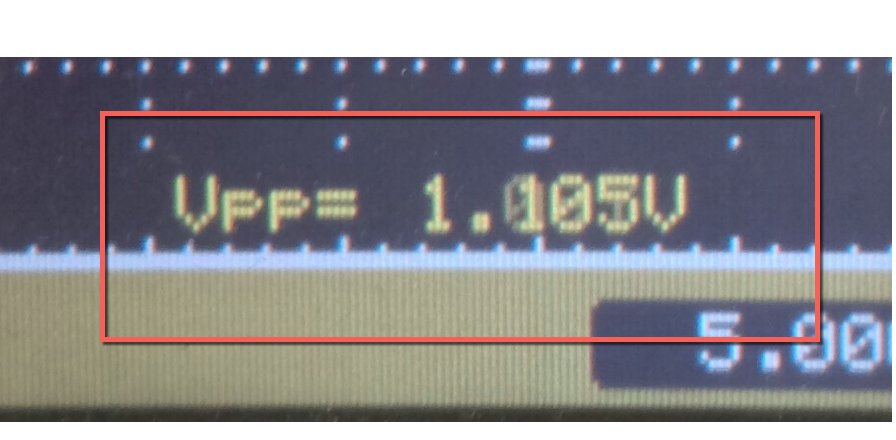
\includegraphics[scale = 0.4]{vpp.png}
\captionof{figure}{Amplitude real time measurement. Vpp is at around 1v.}
\end{minipage}
\medskip
\end{center}

A table from this program is also implemented which can be seen from section \ref{sec:amp}

\subsubsection{Matlab code for setting up refresh rate}
\label{sec:refresh}
This code enable us to calculate how much delay is needed to change the refresh rate down to 50hz:
\begin{lstlisting}[language=Verilog]
x = 160;
y = 120;
f = 25*10^6;
t = 1/f;

screen_time = t*x*y;
line_time = t*x;


freq = 48;
one_hz_time = 1/freq;
disp(['to draw a whole screen:',num2str(screen_time) ]);
disp(['to draw a whole line:',num2str(line_time) ]);
disp(['to delay at ',num2str(freq),'hz. 25Mhz needed(positive edge): ',num2str(one_hz_time/t),'. bit needed ',num2str(ceil(log2(one_hz_time/t)))]);
\end{lstlisting}

And it is the output:
\begin{verbatim}
to draw a whole screen:0.000768
to draw a whole line:6.4e-06
to delay at 48hz. 25Mhz needed(positive edge): 520833.3333. bit needed 19
\end{verbatim}

\subsubsection{Matlab code for calculating biased shift}

\label{sec:biased}
Because the center of the AD data is at $01\_111\_111\_111\_111$ and our screen's center is at 60. We need to balance the bias by introducing some artificial biases, 
\begin{lstlisting}[language=Matlab]
tk = [1];
original = repmat(tk,1,13);
display('the original center')
bi2de(original)

for i = 3:11
    now_center = bi2de(original(1:end-i));
    if now_center-60 > 0
        bit_needed=ceil(log2(now_center)+1);
        sign = 'plus';
    else
        bit_needed=ceil(log2(60- now_center));
        sign = 'negative';
    end
    display(['shift by ',num2str(i),', to bias it ',sign,' ',num2str(now_center-59)])
end
\end{lstlisting}
And it is the output:
\begin{verbatim}
shift by 3, to bias it plus 964
shift by 4, to bias it plus 452
shift by 5, to bias it plus 196
shift by 6, to bias it plus 68
shift by 7, to bias it plus 4
shift by 8, to bias it negative -28
shift by 9, to bias it negative -44
shift by 10, to bias it negative -52
shift by 11, to bias it negative -56
\end{verbatim}

\section{Module Specification}

Below is the list of modules I implemented, besides from this are some Mega function modules.
\subsection{VGA Module}
VGA module is simply the implementation of the module in section \ref{sec:vga}.
\subsection{AD-DA Module}
\paragraph{AD module}
AD module is simply the module from section \ref{sec:adda}. 
\paragraph{DA module}

DA module is combined in two parts, first one is the module from section \ref{sec:adda}. And then a simple counter \ref{sec:signalgenv} is implemented to keep recording of the value of the push button. The system will change its output wave according to this value.

\subsection{State Machine Module}
\label{sec:statusm}
State machine \ref{sec:displaystatev} is combined in 4 parts, which can be seen from section \ref{sec:back}, section \ref{sec:wave}, section \ref{sec:fill} and section \ref{sec:pause}. And the implementation of controlling part is in section \ref{sec:status}. Besides from which, it also has a built in dual port RAM for section \ref{sec:wave} to read and section \ref{sec:fill} to write.
\subsection{Drawing Background Module}
This is an implementation \ref{sec:clearv} of section \ref{sec:coucount}. And it also has a built in RAM which stores the background image. The source code is in \ref{sec:clearv}
\label{sec:back}

\subsection{Drawing Wave Module}
This is an implementation \ref{sec:vgasinv} of section \ref{sec:bascount} for providing X coordinate and \ref{sec:jumcount} for providing RAM reading address. By adding the input value it also supports shift.
\label{sec:wave}

\subsection{Storing AD Data Module}
This is an implementation \ref{sec:ramfilllv} of section \ref{sec:bascount} for providing RAM writing address and an implementation of section \ref{sec:trigger} for supporting triggering and an implementation of section \ref{sec:duram} for section \ref{sec:statusm} to detects its behaviour in reading cycle.
\label{sec:fill}

\subsection{Pause Module}
This is an implementation \ref{sec:delayv} of the section \ref{sec:bascount} to simply cause a delay to scale down the refresh rate at around 50hz. The counter's value is calculated by section \ref{sec:refresh}.
\label{sec:pause}

\subsection{Sampling rate switch module}

This module \ref{sec:selclkv} is simply to change its output frequency according to the switches value. The input frequencies are generated by PLL. 

\subsection{Resize module}

This module \ref{sec:modisignv} is simply to resize the input by doing bits shift, and the bias value can be found in section \ref{sec:biased}

\section{Conclusion and potential works}

For this project I learnt the advantage and constraints of the FPGA developement. The advantage is the FPGA is not programming and by natrual it is in parallel. But due to it is a description of the connitivity of the hardware rather than an explicit description of human login the implementation of an algorithm generaly is harder than a modern programming language. 

Below is a list of potential works:
\begin{itemize}
\item It would be great if we can use a \textit{soft core} and use C or Handel C along with Verilog HDL programming language.

\item According to \textit{quartus}, my design has used 67\% of the memory and 31\% of pins, total login elements consummation is at around 2\%. Colorful background is not possible due to the restriction of the RAM. But we may can implement the design at a higher resolution.\\


\item By implementation more trigger, we will be able to detect the value of the wave(i.e. frequency, amplitude) by the board itself and we can further exploit the functionality of the LCD to show the value.\\

\item Only one route of the AD is implemented, if time allowing, it is possible to change into two route.\\

\item By pining out the trigger to pin EXT\_CLOCK, we can use external to trigger out plotting.
\end{itemize}

 
\section{Appendix}

\subsection{Frequency Table}
\label{sec:fre}
The first column is for switch 14-13 and the second one is for switch 12-11.\\

\begin{minipage}{.5\linewidth}
\begin{tabular}{p{0.3cm}|p{0.3cm}| p{1.2cm}|p{1.2cm}|p{1.2cm}|p{1.2cm}|p{1.2cm}|p{1.2cm}|p{1.2cm}|p{1.2cm}|p{1.2cm}|p{1.2cm}}

&& 1 & 2 & 3 & 4 & 5 & 6 & 7 & 8 & 9 &10 \\ \hline


10&00&84375&168750&253125&337500&421875&506250&590625&675000&759375&843750\\ \hline




10&01&42187.5&84375&126562.5&168750&210937.5&253125&295312.5&337500&379687.5&421875\\ \hline




10&10&28125&56250&84375&112500&140625&168750&196875&225000&253125&281250\\ \hline




10&11&21093.75&42187.5&63281.25&84375&105468.75&126562.5&147656.25&168750&189843.75&210937.5\\ \hline




01&00&337500&675000&1012500&1350000&1687500&2025000&2362500&2700000&3037500&3375000\\ \hline




01&01&168750&337500&506250&675000&843750&1012500&1181250&1350000&1518750&1687500\\ \hline




01&10&112500&225000&337500&450000&562500&675000&787500&900000&1012500&1125000\\ \hline




01&11&84375&168750&253125&337500&421875&506250&590625&675000&759375&843750\\ \hline




11&00&168750&337500&506250&675000&843750&1012500&1181250&1350000&1518750&1687500\\ \hline




11&01&84375&168750&253125&337500&421875&506250&590625&675000&759375&843750\\ \hline




11&10&56250&112500&168750&225000&281250&337500&393750&450000&506250&562500\\ \hline


11&11&42187.5&84375&126562.5&168750&210937.5&253125&295312.5&337500&379687.5&421875\\ 
\end{tabular}
\end{minipage}

\subsection{Amplitude Table}
\label{sec:amp}
\begin{center}
\begin{tabular}{cccc}
switch4-1& one grid & two grid & three grid\\ \hline 
0000&0.63492&1.2698&1.9048\\ \hline




0001&1.2903&2.5806&3.871\\ \hline




0010&2.6667&5.3333&8\\ \hline




0011&5.7143&11.4286&17.1429\\ \hline




0100&0.31496&0.62992&0.94488\\ \hline




1000&0.15686&0.31373&0.47059\\ \hline




1100&0.078278&0.15656&0.23483\\ \hline
\end{tabular}
\end{center}


\subsection{Development History}
\begin{longtable}{@{\extracolsep{\fill}}lll@{}}
Writer & Date & Commit \\
Yingjie & 2015-04-01 & Initial commit \\ \hline
Yingjie & 2015-04-01 & git ignore \\ \hline
Yingjie & 2015-04-01 & .gitignore is now working \\ \hline
Yingjie & 2015-04-01 & Error gitignore fixed \\ \hline
Yingjie & 2015-04-02 & 1 bit ram success \\ \hline
Yingjie & 2015-04-02 & now it is a moving images, but it is correct, may have to do with the address\_max \\ \hline
Yingjie & 2015-04-07 & Edge from negative to positive \\ \hline
Yingjie & 2015-04-07 & Adding matlab source code for black and white image \\ \hline
Yingjie & 2015-04-07 & Now it is static image \\ \hline
Yingjie & 2015-04-07 & From manual address to mulitiplication \\ \hline
Yingjie & 2015-04-07 & Clear module removed, working on sine module \\ \hline
Yingjie & 2015-04-07 & Now this module can draw a sine wave \\ \hline
Yingjie & 2015-04-07 & add the matlab .mif generator \\ \hline
Yingjie & 2015-04-21 & Delete vga to lcd \\ \hline
Yingjie & 2015-04-21 & ADC AND VGA \\ \hline
Yingjie & 2015-04-21 & working on state machine \\ \hline
Yingjie & 2015-04-21 & Starting on state machine from vga+adc and two ms \\ \hline
Yingjie & 2015-04-21 & Removed previous display module, testing sinewave with lock \\ \hline
Yingjie & 2015-04-21 & lock success \\ \hline
Yingjie & 2015-04-21 & Suggestted LCD\_VGA.bdf file, only ad, leave the display vacant \\ \hline
Yingjie & 2015-04-21 & testing state machine \\ \hline
Yingjie & 2015-04-21 & testing on transfer inputs \\ \hline
Yingjie & 2015-04-21 & A initial value bug \\ \hline
Yingjie & 2015-04-21 & bug, only last item works \\ \hline
Yingjie & 2015-04-21 & Now a configurable sine wave, sw1: a bug to be solved \\ \hline
Yingjie & 2015-04-21 & Bug fixed, sw16 to draw sine or not \\ \hline
Yingjie & 2015-04-21 & Remove bug in sine display, moving on state machine \\ \hline
Yingjie & 2015-04-21 & Now at the same time \\ \hline
Yingjie & 2015-04-21 & New image overlapping \\ \hline
Yingjie & 2015-04-21 & A static image overlapping \\ \hline
Yingjie & 2015-04-21 & static image,perfect sequence \\ \hline
Yingjie & 2015-04-21 & Now a static overlapping image with a good background \\ \hline
Yingjie & 2015-04-22 & State machine merged \\ \hline
Yingjie & 2015-04-22 & Now connected to vga, working on trigger \\ \hline
Yingjie & 2015-04-22 & blank initial screen \\ \hline
Yingjie & 2015-04-23 & temp\_commit \\ \hline
Yingjie & 2015-04-24 & reverted to state machine \\ \hline
Yingjie & 2015-04-24 & background,sin\_draw now is state\_machine, wokring on introduce adc using fifo \\ \hline
Yingjie & 2015-04-24 & Introduce test bench using iverilog \\ \hline
Yingjie & 2015-04-24 & state machine for delay,sin\_show,clean,woking on fifo \\ \hline
Yingjie & 2015-04-24 & Add mif file back \\ \hline
Yingjie & 2015-04-24 & Now switch with led on, changed LCM\_VGA.bdf file \\ \hline
Yingjie & 2015-04-24 & first fifo mapper \\ \hline
Yingjie & 2015-04-24 & Added a always writing adc to the module under draw\_sin, going to implement trigger \\ \hline
Yingjie & 2015-04-24 & Now I can see from the vga, woking on trigger and data\_mapper \\ \hline
Yingjie & 2015-04-24 & Now the waveform is in the center \\ \hline
Yingjie & 2015-04-25 & Temp commit at 25 April \\ \hline
Yingjie Luan & 2015-04-26 & working on manual ram, fifo is too complicated \\ \hline
Yingjie Luan & 2015-04-26 & finished writing manually ram \\ \hline
Yingjie Luan & 2015-04-26 & Successeed \\ \hline
Yingjie Luan & 2015-04-26 & `reset' bug fixed by change the default status to do\_nothing \\ \hline
Yingjie Luan & 2015-04-26 & synthesis adc clock \\ \hline
Yingjie Luan & 2015-04-26 & working on synchonzing finished signal \\ \hline
Yingjie Luan & 2015-04-26 & Sync Proved success \\ \hline
Yingjie Luan & 2015-04-26 & change background \\ \hline
Yingjie Luan & 2015-04-26 & Rename trigger module into sample time \\ \hline
Yingjie Luan & 2015-04-26 & trigger enabled, but image not still \\ \hline
Yingjie Luan & 2015-04-26 & changed a trigger design, still not working \\ \hline
Yingjie Luan & 2015-04-26 & The clock changer is wrong,now a static image \\ \hline
Yingjie Luan & 2015-04-26 & trigger with new design \\ \hline
Yingjie Luan & 2015-04-26 & Pin out state and clock, not functioning \\ \hline
Yingjie Luan & 2015-04-26 & Functioning with new trigger \\ \hline
Yingjie Luan & 2015-04-26 & Merge branch `new\_compressor' \\ \hline
Yingjie Luan & 2015-04-26 & Added a converter module \\ \hline
Yingjie Luan & 2015-04-26 & Changed default state \\ \hline
Yingjie Luan & 2015-04-27 & Update Matlab Function \\ \hline
Yingjie Luan & 2015-04-29 & 3 sample clock \\ \hline
Yingjie Luan & 2015-04-29 & Implemented sample clock \\ \hline
Yingjie Luan & 2015-04-29 & Merged signal generator \\ \hline
Yingjie Luan & 2015-04-29 & Sample more data \\ \hline
Yingjie Luan & 2015-04-29 & Working on time division \\ \hline
Yingjie Luan & 2015-04-29 & time division \\ \hline
Yingjie Luan & 2015-04-29 & MOVE up and down \\ \hline
Yingjie Luan & 2015-04-29 & rescale \\ \hline
Yingjie Luan & 2015-04-29 & Multiple waves signal generator \\ \hline
Yingjie Luan & 2015-04-29 & Update wave \\ \hline
Yingjie Luan & 2015-04-29 & Signal\_selector\_without\_test \\ \hline\end{longtable}

\subsection{Full Source Code}
\subsubsection{clear.v}
\label{sec:clearv}
\begin{lstlisting}[language=Verilog]
module clear(CounterX,CounterY,clk,reset,enable,finished,color);

input clk;
input reset,enable;

output reg [7:0] CounterX,CounterY;
output finished;

wire [14:0] address;

wire CounterXmaxed = (CounterX==8'd159); // 159
wire CounterYmaxed = (CounterY==8'd119); // 119
assign finished = ((CounterXmaxed == 1) && (CounterYmaxed == 1));

assign address = CounterX + CounterY * 160;

always @(posedge clk)
begin
  if(reset == 1)
    CounterX <= 0;
  else
  begin
  if(CounterXmaxed)
    CounterX <= 0;
  else if(enable == 1)
    CounterX <= CounterX + 1;
  end
end

always @ (posedge clk)
begin
  if(reset == 1)
    CounterY <= 0;
  else
  begin
    if(CounterXmaxed == 1)
    begin
      if(CounterYmaxed)
        CounterY <= 0;
      else if(enable == 1)
        CounterY <= CounterY + 1;
    end
  end
end

// output color;
// endmodule


output [11:0] color = {12{rambuffer}};
wire rambuffer;
ram_background ram_entity(
  .address(address),
  .clock(clk),
  .wren(1'b0),
  .q(rambuffer));

endmodule
\end{lstlisting}

\subsubsection{delay.v}
\label{sec:delayv}
\begin{lstlisting}[language=Verilog]
module delay(clk,enable,reset,finished);

// module vga_sin(CounterX,CounterY,color,clk,enable,reset,finished);

// to draw a whole screen:0.000768
// to draw a whole line:6.4e-06
// to delay at 48hz rate:0.02083325mhz needed(positive edge)520833.3333

input clk,enable,reset;
output finished;

parameter cycle = 'd520833;

reg [19:0] counter; // log2(520833.333) ~= 19
wire countermaxed = (counter == cycle);
assign finished = countermaxed;

always @(posedge clk)
begin
  if(reset == 1)
    counter <= 0;
  else
  begin
  if(countermaxed)
      counter <= 0;
  else if(enable == 1)
      counter <= counter + 1;
  end
end

endmodule
\end{lstlisting}

\subsubsection{display\_state.v}
\label{sec:displaystatev}
\begin{lstlisting}[language=Verilog]
// module display_state(CounterX,CounterY,color,clk,clk_en,rst_n);
module display_state(CounterX,CounterY,color,clk,clk_en,rst_n,
  adc_data,clk_adc,state,clk_down,vga_data,time_division,
  move_up,move_down);

input clk;
input clk_en,rst_n;//clk_en is not implemented

output reg [7:0] CounterX,CounterY;
output reg [11:0] color;

// module vga_sin(CounterX,CounterY,color,clk,enable,reset,finished);
// module clear(CounterX,CounterY,clk,reset,enable,finished,color);
wire [7:0] CounterX_clear,CounterY_clear,CounterX_sin;
wire [11:0] color_clear, color_sin;
reg enable_clear,enable_sin,reset_clear,reset_sin,enable_delay,reset_delay;
wire finished_clear,finished_sin,finished_delay;

input [2:0] move_up,move_down;

sample_clock htime_entity(
  .clk_in(clk_adc),
  .clk_out(clk_down));
// ram_flash ram_entity(
//   .data(data_flash_reg), .wraddress(wraddress), .wren(Acquiring), .wrclock(clk_flash),
//   .q(ram_output), .rdaddress(rdaddress), .rden(rden), .rdclock(clk)
// );
wire [7:0] ram_output;
input [7:0] vga_data;//= (adc_data >> 7)-4;

input [13:0] adc_data;
input clk_adc;

manual_ram ram_entity(
  .data(vga_data), .wraddress(CounterX_fill),.wren(write_enable),.wrclock(clk_down), 
  .q(ram_output), .rdaddress(read_CounterX_sin),.rden(enable_sin),.rdclock(clk));

// module ramfill(clk_adc,enable,reset,finished,CounterX);

reg enable_fill,reset_fill;
wire finished_fill;
wire [10:0] CounterX_fill;
output wire clk_down;

wire write_enable;
ramfill fill_module(
  .clk_adc(clk_down),
  .enable(enable_fill),
  .reset(reset_fill),
  .clk(clk),
  .adc_data(adc_data),
  .r_finished(finished_fill),
  .write_enable(write_enable),
  .CounterX(CounterX_fill));

clear clear_module(
  .CounterX(CounterX_clear),
  .CounterY(CounterY_clear),
  .color(color_clear),
  .clk(clk),
  .enable(enable_clear),
  .reset(reset_clear),
  .finished(finished_clear));

// module vga_sin(CounterX,CounterY,color,clk,enable,reset,finished,clk_adc,adc_data);
input [1:0] time_division;
wire [10:0] read_CounterX_sin;
vga_sin sin_module(
  .CounterX(CounterX_sin),
  .color(color_sin),
  .clk(clk),
  .enable(enable_sin),
  .reset(reset_sin),
  .read_CounterX(read_CounterX_sin),
  .time_division(time_division),
  .finished(finished_sin));

delay delay_module(
  .clk(clk), 
  .enable(enable_delay),
  .reset(reset_delay), 
  .finished(finished_delay));
//  defparam delay_module.cycle ='d10008;

parameter [1:0] clear_screen = 2'b00, draw_line = 2'b01, do_nothing = 2'b10, fill = 2'b11;

output reg [1:0] state;
reg [1:0] next_state;

initial begin
  state = clear_screen;
end

always @ (posedge clk)
begin
  if(rst_n == 1)
    state <= clear_screen;
  else
    state <= next_state;
end

always @ * // combinational circuit
  case(state)
    clear_screen:
    begin
      enable_clear = 1;
      reset_clear = 0;

      enable_sin = 0;
      reset_sin = 1;

      enable_delay = 0;
      reset_delay = 1;

      enable_fill = 0;
      reset_fill = 1;

      CounterX = CounterX_clear;
      CounterY = CounterY_clear;
      color = color_clear;
      if(finished_clear == 0)
        next_state = clear_screen;
      else
        next_state = fill;
    end
    fill:
    begin
      enable_fill = 1;
      reset_fill = 0;   

      enable_clear = 0;
      reset_clear = 1;

      enable_sin = 0;
      reset_sin = 1;

      enable_delay = 0;
      reset_delay = 1;

      CounterX = 8'bzzzz_zzz;
      CounterY = 8'bzzzz_zzz;
      color = 12'bzzz_zzz_zzz_zzz;

      if(finished_fill == 0)
        next_state = fill;
      else
        next_state = draw_line;     

    end
    draw_line:
    begin
      enable_sin = 1;
      reset_sin = 0;

      enable_delay = 0;
      reset_delay = 1;

      enable_clear = 0;
      reset_clear = 1;

      enable_fill = 0;
      reset_fill = 1;     

      CounterX = CounterX_sin;
      CounterY = ram_output + move_down - move_up;
      color = color_sin;
      if(finished_sin == 0)
        next_state = draw_line;
      else
        next_state = do_nothing;
    end
    do_nothing:
    begin
      enable_delay = 1;
      reset_delay = 0;

      enable_clear = 0;
      reset_clear = 1;

      enable_sin = 0;
      reset_sin = 1;

      enable_fill = 0;
      reset_fill = 1;     

      CounterX = 8'bzzzz_zzz;
      CounterY = 8'bzzzz_zzz;
      color = 12'bzzz_zzz_zzz_zzz;
      if(finished_delay == 0)
        next_state = do_nothing;
      else  
        next_state = clear_screen;
    end 
  endcase

endmodule

\end{lstlisting}

\subsubsection{modisign.v}
\label{sec:modisignv}
\begin{lstlisting}[language=Verilog]
module modisign(adc_data,vga_data,shift);

// horizonal resize 
input [13:0] adc_data;
output reg [7:0] vga_data;

input [3:0] shift; // 0, 1, 2, 3
// matlab function provided for calculate bits real shift 


// original center is 8191 {13[1]}, the center shift as well.
always @ *
begin
  case(shift)
  0:
  begin
    vga_data = (adc_data >> 7) - 4 ;
  end
  1:
  begin
    vga_data = (adc_data >> 8) + 28 ;
  end
  2:
  begin
    vga_data = (adc_data >> 9) + 44 ;
  end
  3:
  begin
    vga_data = (adc_data >> 10) + 52 ;
  end
  4:
  begin
    vga_data = (adc_data >> 6) - 68 ;
  end
  8:
  begin
    vga_data = (adc_data >> 5) - 196 ;
  end
  12:
  begin
    vga_data = (adc_data >> 4) - 452 ;
  end
  default:
  begin
    vga_data = (adc_data >> 7) - 4 ;
  end

  endcase
end
// values of data_shift :( as resolution goes lower
// shift by 7: 4
// shift by 8:

endmodule
\end{lstlisting}

\subsubsection{ramfill.v}
\label{sec:ramfilllv}
\begin{lstlisting}[language=Verilog]
// module ramfill(clk_adc,enable,reset,finfished,adc_data,vga_data);
module ramfill(clk_adc,enable,reset,r_finished,adc_data,CounterX,clk,write_enable);

input clk_adc,clk;
input enable,reset;
input [13:0] adc_data;
output reg write_enable;
output reg r_finished;


wire last_bit_data = adc_data[13];
reg previous_adc_data;

// wait until trigger happen
always @ (posedge clk_adc)
begin
  previous_adc_data <= last_bit_data;
  if(enable == 1)
  begin
    if(Trigger == 1) // unchanged until enable returns to 0.
      write_enable <= 1;
  end
  else
    write_enable <= 0;
end

reg Threshold1, Threshold2;
always @(posedge clk_adc) Threshold1 <= (adc_data>=14'b10_000_000_000_000);
always @(posedge clk_adc) Threshold2 <= Threshold1;

wire Trigger = Threshold1 & ~Threshold2;  // if positive edge, trigger! 


// sync clocks
reg prolong_finished = 0;
always @(posedge w_finished)
begin
  prolong_finished = prolong_finished + 1;
end

reg previous_signal;
always @(posedge clk) // flip flop
begin
  previous_signal <= prolong_finished; 
  r_finished <= previous_signal ^ prolong_finished;
  // or with its previous value.
end


// build a 160 counter
output reg [10:0] CounterX;

wire CounterXmaxed = (CounterX=='d2047); // 2048 words for late down sampling
wire w_finished;
assign w_finished = (CounterXmaxed==1);


always @(posedge clk_adc)
begin
  if(reset == 1)
    CounterX <= 0;
  else
  begin
  if(CounterXmaxed)
      CounterX <= 0;
  else if(write_enable == 1)
      CounterX <= CounterX + 1;
  end
end

endmodule

\end{lstlisting}

\subsubsection{vga\_sin.v}
\label{sec:vgasinv}
\begin{lstlisting}[language=Verilog]
module vga_sin(CounterX,color,clk,enable,reset,finished,read_CounterX,time_division);
// module vga_sin(CounterX,CounterY,color,clk,enable,reset,finished);
// module vga_sin(CounterX,CounterY,color,clk,enable,reset,finished,clk_adc,adc_data);


input clk;
input enable,reset;
input [1:0] time_division;
wire [2:0] read_time_division = time_division + 1; // to avoid 0, start from 1

output finished;
output reg [7:0] CounterX;
output [11:0] color;

 
assign color = 12'hF00; // color to be drawn

wire CounterXmaxed = (CounterX==8'd159); // 159
assign finished = (CounterXmaxed==1);

always @(posedge clk)
begin
  if(reset == 1)
    CounterX <= 0;
  else
  begin
  if(CounterXmaxed)
      CounterX <= 0;
  else if(enable == 1)
      CounterX <= CounterX + 1;
   end
end

output reg [10:0] read_CounterX;
wire read_CounterX_Maxed = (read_CounterX >= 'd2047);
always @(posedge clk)
begin
  if(reset == 1)
    read_CounterX <= 0;
  else
  begin
  if(read_CounterX_Maxed)
      read_CounterX <= 0;
  else if(enable == 1)
      read_CounterX <= read_CounterX + read_time_division;
   end
end

// endmodule

// module collect_data(clk_adc,enable,reset,finished,data_in,data_out,read_busy);
// input clk_adc;
// input [13:0] adc_data;

// output [7:0] CounterY;

// // for the moment, the fifo will read the data when the drawer is off continously until full. The word length is not
// // correct as well, it 128 instead of 120.. Going to implmented the trigger after testing the adc
// //module collect_data(clk_adc,clk,enable,reset,finished,data_in,data_out,read_busy);

// collect_data fifo_entity(
//  .clk_adc(clk_adc),
//  .clk(clk),
//  .data_in(adc_data),
//  .data_out(CounterY), 
//  .read_busy(~enable)); //"when enabled it is busy to draw on the screen, usually, enable is the opposite of reset and finifhsed
  
endmodule

\end{lstlisting}

\subsubsection{sel\_clk.v}
\label{sec:selclkv}
\begin{lstlisting}[language=Verilog]
module sel_clk(clk1,clk2,clk3,in_p,clk_62);

input clk1,clk2,clk3;
input [1:0] in_p;

output reg clk_62;

always @(in_p)
begin
  case(in_p)
    'd0:clk_62 = clk1;
    'd1:clk_62 = clk2;
    'd2:clk_62 = clk3;
    default: clk_62 = clk1;
  endcase
end

endmodule
\end{lstlisting}

\subsubsection{signal\_gen.v}
\label{sec:signalgenv}
\begin{lstlisting}[language=Verilog]
module sign_gen(clk_dac,value,enable,reset,finished,switch);

input clk_dac;
input enable,reset;
output finished;


// 4 ram block with different initial momeory.
sin_test sin_entity(
  .address(CounterX),
  .clock(clk_dac),
  .wren(1'b0), 
  .q(val1));
sin_test1 sin_entity1(
  .address(CounterX),
  .clock(clk_dac),
  .wren(1'b0), 
  .q(val2));
sin_test2 sin_entity2(
  .address(CounterX),
  .clock(clk_dac),
  .wren(1'b0), 
  .q(val3));
sin_test3 sin_entity3(
  .address(CounterX),
  .clock(clk_dac),
  .wren(1'b0), 
  .q(val4));

sin_test1 sin_entity1(
  .address(CounterX),
  .clock(clk_dac),
  .wren(1'b0), 
  .q(val2));

sin_test2 sin_entity2(
  .address(CounterX),
  .clock(clk_dac),
  .wren(1'b0), 
  .q(val3));

sin_test3 sin_entity3(
  .address(CounterX),
  .clock(clk_dac),
  .wren(1'b0), 
  .q(val4));




input switch;
reg [1:0] re_switch;

wire [13:0] val1,val2,val3,val4;
output reg [13:0] value;

initial
begin
  re_switch <= 'b00;
end

always @ (posedge switch)
  re_switch <= re_switch + 1'b1;

always @ *
  case(re_switch)
  'b00:
  value = val1;
  'b01:
  value = val2;
  'b10:
  value = val3;
  'b11:
  value = val4;
  endcase






reg [9:0] CounterX;
// a 1024 counter
// module vga_sin(CounterX,color,clk,enable,reset,finished,read_CounterX,time_division);
wire CounterXmaxed = (CounterX=='d1023); // samples 1024
wire finished;
assign finished = (CounterXmaxed==1);


always @(posedge clk_dac)
begin
  if(reset == 1)
    CounterX <= 0;
  else
  begin
  if(CounterXmaxed)
      CounterX <= 0;
  else if(enable == 1)
      CounterX <= CounterX + 1;
  end
end

endmodule

\end{lstlisting}

\bibliographystyle{plain}
\bibliography{bibliography} 
\end{document}
